\catcode"200B=9
\documentclass[zihao=-4]{ctexart}
\usepackage[normalem]{ulem}
\useunder{\uline}{\ul}{}
%********************导言区宏包引入********************
\usepackage{xeCJK}
\usepackage{graphicx}
\usepackage{eso-pic}
% 整页图片命令：用于第一页
\newcommand{\FullPageImage}[1]{%
  \thispagestyle{empty}%
  \AddToShipoutPictureBG*{%
    \AtPageLowerLeft{%
      \includegraphics[width=\paperwidth,height=\paperheight]{#1}%
    }%
  }%
  \null
  \clearpage
}

% 后续页面背景图命令：从调用之后的页面开始生效
\newcommand{\SetPageBackground}[1]{%
  \AddToShipoutPictureBG{%
    \AtPageLowerLeft{%
      \includegraphics[width=\paperwidth,height=\paperheight]{#1}%
    }%
  }%
}
\usepackage{amssymb}
\usepackage{amsmath}
\usepackage{listings} %代码
\usepackage{graphicx}
\usepackage{float}
\usepackage{multicol} %回车换段
\usepackage{xcolor}
\usepackage{geometry} %页面设置
\usepackage{fontspec}
\usepackage{setspace}
\usepackage{array}
\usepackage{enumitem}
\usepackage{comment}
\usepackage{tabularx}
\usepackage{fancyhdr} %页眉页脚
\usepackage{xurl} %允许长 URL 在斜杠、下划线等位置断行
\urlstyle{same} % URL 沿用正文衬线字体
\pagestyle{fancy}
\setlength{\headheight}{15pt}
\usepackage{float} %表格位置
\usepackage{titlesec} %设置
\usepackage{titletoc}
\usepackage{gbt7714}    %控制参考文献格式为国标
\usepackage{multirow}
\usepackage{float}
\usepackage{booktabs}   %表格相关
\usepackage{setspace}   %设置行距
\usepackage{caption} %caption
\usepackage{subcaption} %子图的caption
\usepackage{changepage} %左右缩进
\usepackage{pifont} %带圆圈标号
\usepackage{subcaption}
\usepackage{caption}

%********************Unicode 字符兼容处理********************
% 解决 XeLaTeX 下 Times New Roman / 数学字体缺少 Unicode 希腊字母、特殊符号的问题
\usepackage{newunicodechar}

\newunicodechar{α}{\ensuremath{\alpha}}
\newunicodechar{β}{\ensuremath{\beta}}
\newunicodechar{γ}{\ensuremath{\gamma}}
\newunicodechar{δ}{\ensuremath{\delta}}
\newunicodechar{ε}{\ensuremath{\varepsilon}}
\newunicodechar{η}{\ensuremath{\eta}}
\newunicodechar{θ}{\ensuremath{\theta}}
\newunicodechar{λ}{\ensuremath{\lambda}}
\newunicodechar{μ}{\ensuremath{\mu}}
\newunicodechar{σ}{\ensuremath{\sigma}}
\newunicodechar{ρ}{\ensuremath{\rho}}
\newunicodechar{τ}{\ensuremath{\tau}}
\newunicodechar{φ}{\ensuremath{\varphi}}
\newunicodechar{ϕ}{\ensuremath{\varphi}}
\newunicodechar{ω}{\ensuremath{\omega}}
\newunicodechar{ó}{\'o}
\newunicodechar{í}{\'i}
\newunicodechar{ö}{\"o}
\newunicodechar{́}{}
\newunicodechar{̈}{}
\newunicodechar{Δ}{\ensuremath{\Delta}}
\newunicodechar{Ω}{\ensuremath{\Omega}}
\newunicodechar{×}{\ensuremath{\times}}
\newunicodechar{·}{\ensuremath{\cdot}}
\newunicodechar{√}{\ensuremath{\checkmark}}
\newunicodechar{≤}{\ensuremath{\le}}
\newunicodechar{≥}{\ensuremath{\ge}}
\newunicodechar{→}{\ensuremath{\rightarrow}}
% 处理误写在数学模式中的中文顿号，如 $x、y、z$
\newunicodechar{、}{\ifmmode\text{、}\else\symbol{"3001}\fi}
%********************Unicode 字符兼容处理********************

\graphicspath{ {include_picture/} }
\let\algorithm\relax
\let\endalgorithm\relax
\usepackage[ruled,vlined]{algorithm2e}%[ruled,vlined]{
\usepackage{algpseudocode}
\renewcommand{\algorithmicrequire}{\textbf{Input:}} 
\renewcommand{\algorithmicensure}{\textbf{Output:}}
%\renewcommand\thepage{\zihao{-5} ~\arabic{page}~}%页码字号

%定义两个arg
\DeclareMathOperator*{\argmax}{arg\,max}
\DeclareMathOperator*{\argmin}{arg\,min}
\DeclareCaptionLabelSeparator{mysep}{\space\space}  %自定义caption格式
\captionsetup[figure]{font={small}, labelfont=bf, labelsep=mysep, textfont=bf}   %图片caption格式
\captionsetup[table]{font={small}, labelfont=bf, labelsep=mysep, textfont={bf}}   %表格caption格式
\bibliographystyle{gbt7714-numerical} %修改了title斜体内容

%********************导言区宏包引入********************
%********************第三方字体引入********************
%\setCJKmainfont[Path=fonts/,BoldFont=simhei.ttf,ItalicFont=simkai.ttf,SlantedFont=simfang.ttf]{simsun.ttc}
%中文字体涵盖黑体、宋体、楷体、仿宋
\setmainfont[Path=fonts/, 
BoldFont = times-new-roman-bold.ttf,
ItalicFont = times-new-roman-italic.ttf,
BoldItalicFont = times-new-roman-bold-italic.ttf
]{times-new-roman.ttf}
\setmonofont[Path=fonts/]{Courier New.ttf}
\setCJKfamilyfont{hwzs}[Path=fonts/]{STKzhongsong.ttf}%使用STZhogsong华文中宋字体
\newcommand{\zhongsong}{\CJKfamily{hwzs}}
\setCJKfamilyfont{hwxw}[Path=fonts/]{STKxinwei.ttf} % XSP 2023/3/3:
\newcommand{\xinwei}{\CJKfamily{hwxw}}              %  使用STZxinwei华文新魏字体.

%********************第三方字体引入********************


%********************中文字号设置********************
%\newcommand{\chuhao}{\fontsize{42pt}{\baselineskip}\selectfont}
\newcommand{\chuhao}{\fontsize{42pt}{0}}
\newcommand{\xiaochu}{\fontsize{36pt}{0}}
\newcommand{\yihao}{\fontsize{28pt}{0}}
\newcommand{\erhao}{\fontsize{21pt}{0}}
\newcommand{\xiaoer}{\fontsize{18pt}{0}}
\newcommand{\sanhao}{\fontsize{16pt}{0}}
\newcommand{\sihao}{\fontsize{14pt}{0}}
\newcommand{\xiaosi}{\fontsize{12pt}{0}}
\newcommand{\wuhao}{\fontsize{10.5pt}{0}}
\newcommand{\xiaowu}{\fontsize{9pt}{0}}
\newcommand{\liuhao}{\fontsize{8pt}{0}}
\newcommand{\qihao}{\fontsize{5.25pt}{0}}
%********************中文字号设置********************


%********************页边距设置********************
\geometry{left=3cm,right=2cm,top=2.5cm,bottom=2.5cm}
\geometry{a4paper} % xsp 2023/3/7: 调整纸张大小为A4
%********************页边距设置********************

%********************段间距设置********************
\newcommand{\setParDis}{\setlength {\parskip} {0pt} }
%请在每部分使用这个
%********************段间距设置********************

%********************

\begin{document}

%********************第一页整页图片封面********************
\FullPageImage{include_picture/first_page.png}

%********************从第二页开始添加背景图********************
\SetPageBackground{include_picture/background.png}

%********************页眉页脚设置********************
\lhead{}
\rhead{}
\setlength{\headwidth}{\textwidth}
%********************页眉页脚设置********************

%********************标题格式设置********************

\setcounter{secnumdepth}{5}
\setcounter{tocdepth}{3}

\renewcommand{\thesection}{\arabic{section}}
\renewcommand{\thesubsection}{\thesection.\arabic{subsection}}
\renewcommand{\thesubsubsection}{\thesubsection.\arabic{subsubsection}}
\renewcommand{\theparagraph}{\thesubsubsection.\arabic{paragraph}}
\renewcommand{\thesubparagraph}{\theparagraph.\arabic{subparagraph}}

\titleformat{\section}[block]
  {\sanhao\heiti\centering}
  {\thesection}
  {1em}
  {}[]

\titleformat{\subsection}[block]
  {\sihao\heiti}
  {\thesubsection}
  {1em}
  {}[]

\titleformat{\subsubsection}[block]
  {\xiaosi\heiti}
  {\thesubsubsection}
  {1em}
  {}[]

\titleformat{\paragraph}[block]
  {\xiaosi\heiti}
  {\theparagraph}
  {0.5em}
  {}[]

\titleformat{\subparagraph}[block]
  {\xiaosi\heiti}
  {\thesubparagraph}
  {0.5em}
  {}[]

\titlespacing{\section}{0pt}{25pt}{12pt}
\titlespacing{\subsection}{0pt}{7pt}{7pt}
\titlespacing{\subsubsection}{0pt}{5pt}{4pt}
\titlespacing{\paragraph}{0pt}{3pt}{2pt}
\titlespacing{\subparagraph}{0pt}{3pt}{2pt}

\titlecontents{section}[1.6em]{\addvspace{2pt}\filright}
{\contentspush{\thecontentslabel\hspace{0.8em}}}
{}{\titlerule*[8pt]{.}\contentspage}

\titlecontents{subsection}[3.2em]{\addvspace{2pt}\filright}
{\contentspush{\thecontentslabel\hspace{0.8em}}}
{}{\titlerule*[8pt]{.}\contentspage}

\titlecontents{subsubsection}[4.8em]{\addvspace{2pt}\filright}
{\contentspush{\thecontentslabel\hspace{0.8em}}}
{}{\titlerule*[8pt]{.}\contentspage}

\linespread{1.8}
\setlength{\parskip}{0.5\baselineskip}

% 摘要页开始
\renewcommand{\headrulewidth}{0pt}
\pagenumbering{roman}

\xiaosi
\section*{摘要}
\begin{spacing}{1.5}
  \setParDis %设置段间距为 0

        孤独症，又称自闭症，是一项终身发展的神经发育型障碍，孤独症患者从出生起，便被一双无形的大手深刻地改变了人生的轨迹。孤独症已成为全球公共卫生领域的重要议题，截至目前，全球约有 6180 万人患有孤独症，约合每 127 人中即有一例，我国现有孤独症确诊患者逾 1300 万，其中年增速超 20 万例，呈现持续攀升态势。

孤独症目前症状未明且无特效药物，鉴于干预工作的专业性，目前由相关机构提供线下一对一干预是孤独症儿童恢复的核心手段。但是仅靠机构干预，孩子的高强度干预难以保证，且高昂的费用让大部分患者家庭在经济天平失衡中负重前行。此外，目前相关机构医患比严重失调且呈现巨大的地区差异性。

为解决上述问题，虚拟现实技术凭借沉浸性、可控性及可重复使用性等优势逐步应用于孤独症干预，但受限于技术其面临三重局限：其一，失真的固定场景加剧孤独症儿童核心障碍——泛化能力缺陷，其二，预设虚拟角色表情等社交要素缺失偏离社交干预本质，其三，患者针对性动态评估体系缺位。这些局限使其训练模式与患者症状的高度异质性形成结构性矛盾，阻碍了技术成果向临床实践的有效转化。

为此，我们提出了北辰——一体化孤独症儿童干预系统，旨在提供个性化的高保真 3D 高斯泼溅场景和高度还原的人物模拟社交场景或干预场景，建立多模态 AI 大模型驱动的智能语音交互系统，对患儿认知功能、社会交往、语言和与表达能力和工具性日常生活能力进行一体化干预训练。此外，北辰系统通过实时数据采集和分析，将复杂神经发育评估转化为可穿戴设备驱动的行为数据分析，为家庭化干预提供客观动态监测锚点，为干预效果提供科学依据，呵护“星星的孩子”健康成长。

 \end{spacing}

\textbf{关键词：}孤独症，干预，虚拟现实，高斯泼溅，大模型对话

\newpage
\section*{\textbf{Abstract}} % XSP 2023/3/8: Abstract 加粗
\begin{spacing}{1.5}
\begin{adjustwidth}{0.42cm}{0.42cm}
    \sloppy
  \setParDis %设置段间距为 0

Autism, also known as autism spectrum disorder, is a lifelong neurodevelopmental disorder. People with autism have had their life trajectories profoundly altered from birth by an invisible force. Autism has become a significant issue in global public health. As of now, approximately 61.8 million people worldwide have autism, which means that about one in every 127 people is affected. In China, there are currently over 13 million confirmed cases of autism, with an annual increase of more than 200,000 cases, showing a continuous upward trend.

Autism currently has unclear symptoms and no specific drugs. Given the professionalism of intervention work, one-on-one offline intervention provided by relevant institutions is currently the core means for the recovery of children with autism. However, relying solely on institutional intervention, it is difficult to ensure the high-intensity intervention for children, and the high cost makes most patient families struggle under the economic imbalance. In addition, the doctor-patient ratio in relevant institutions is seriously imbalanced and shows huge regional differences.

To address the above issues, virtual reality technology, with its advantages such as immersion, controllability and reusability, has gradually been applied in autism intervention. However, due to technical limitations, it faces three major constraints: first, the distorted and fixed scenarios exacerbate the core obstacle of children with autism -- the deficiency in generalization ability; second, the pre-set virtual character expressions and other social elements are missing, deviating from the essence of social intervention; third, the absence of a patient-specific dynamic assessment system. These limitations create a structural contradiction with the high heterogeneity of patient symptoms, hindering the effective transformation of technological achievements into clinical practice.

For this purpose, we have proposed the Beichen -- an integrated intervention system for children with autism, aiming to provide personalized high-fidelity 3D Gaussian splash scenes and highly realistic character simulation social or intervention scenarios. It also establishes a multi-modal AI large model-driven intelligent voice interaction system to conduct integrated intervention training for children’s cognitive functions, social interactions, language and expression abilities, and instrumental activities of daily living. Additionally, the Beichen system converts complex neurodevelopmental assessments into wearable device-driven behavioral data analysis through real-time data collection and analysis, providing objective dynamic monitoring anchor points for family-based intervention and scientific evidence for intervention effects, to care for the healthy growth of ``star children''.

\textbf{Keywords:} Autism, Intervention, Virtual Reality, Gaussan Splatting, Large Language Models
\end{adjustwidth}
\end{spacing}



%********************摘要部分********************


%********************目录部分********************
\clearpage
\tableofcontents
\clearpage
%********************目录部分********************
\renewcommand{\headrulewidth}{0.4pt} %恢复页眉装饰线


\definecolor{headerblue}{RGB}{35,95,170}

%********************正文页眉部分********************
%\lhead{}
\chead{\wuhao 北京航空航天大学第三十五届“冯如杯”竞赛主赛道参赛作品}

%********************正文页眉部分********************

\pagenumbering{arabic} %正文页码从1开始，用阿拉伯数字
\setcounter{page}{1} 

\section{项目背景}
\setParDis %设置段间距为 0
\begin{spacing}{1.5}

\subsection{智慧医疗}

健康中国建设将人民健康置于优先发展的战略位置[1--3]。截至 2026 年 8 月，医疗、康复、教育与残疾人服务正在从单点、线下服务逐步走向以基层为基础、以家庭为重要场景、以连续服务为目标的协同模式。数字技术可将专业人员设计的训练任务、过程记录与随访服务延伸至家庭和城乡社区，为长期干预提供更加连续的技术支持。

2024 年，中国残联、教育部、民政部、国家卫生健康委、国家医保局、共青团中央和全国妇联联合印发《孤独症儿童关爱促进行动实施方案（2024--2028 年）》，提出用约五年时间完善关爱服务工作机制和服务体系，提升孤独症儿童发展全程服务能力与保障条件[51]。在上述政策背景下，面向基层和家庭场景的数字化干预工具，可进一步支持机构训练向家庭和社区延伸，加强康复机构、学校与家庭之间的训练衔接和过程记录。

\subsection{孤独症谱系障碍}

孤独症谱系障碍（Autism Spectrum Disorder，ASD，以下简称孤独症）是一组与脑发育相关的神经发育状况，通常表现为社会沟通和社会互动方面的差异，以及受限、重复的行为、兴趣或活动模式。其临床表现具有较强异质性，可涉及社会沟通、重复或受限行为、感觉加工、语言发展及认知等多个方面。孤独症与大众认知的概念截然不同，大众常误认为孤独症患者对情感无感，实则他们具备丰富的情感体验，只是解读社交信号（如表情、语调）的神经机制异于常人。部分患者甚至会因过度共情而陷入焦虑，这与“冷漠”的标签完全相悖。

此外，刻板动作和特殊兴趣常被污名化为“怪异行为”，实则这些行为具备自我调节功能，例如孤独症的常见症状——“蝴蝶手”，只是患者为了缓解内心的焦虑而产生的外在表现。最新研究指出，规律性重复动作能帮助孤独症患者稳定感知过载的神经系统，其作用类似于人类进化过程中形成的应激保护机制。约 30\% 的孤独症个体存在语言发展迟滞，但语言能力与认知能力和智力之间并不存在简单对应关系。神经影像显示，部分非语言患者在视觉思维、模式识别等领域的脑区活跃度超常，印证了“不同认知方式而非能力缺失”的神经多样性理论。

世界卫生组织 2025 年更新的事实表明，全球 2021 年约每 127 人中有 1 人为孤独症人士；截至 2026 年，国内公开资料显示，我国孤独症人群已超过 1300 万，其中 0--14 岁儿童约 300 万至 500 万[58]。

孤独症儿童的发展轨迹具有较强个体差异，部分个体成年后仍需要持续支持。研究表明，早期识别并及时提供行为干预和教育支持，有助于促进相关能力的发展，亦可在一定程度上缓解家庭的长期照护压力[53]。

我国已形成以早期筛查、转诊、康复训练、学前与学校教育、家庭支持和社会保障共同参与的服务框架。国家卫生健康委发布的《0--6 岁儿童孤独症筛查干预服务规范（试行）》明确了儿童健康管理中的初筛、复筛、转诊和干预服务要求[52]；《孤独症儿童关爱促进行动实施方案（2024--2028 年）》进一步将全程服务能力、教育支持、家庭关爱与社会环境纳入协同治理[51]。上述服务体系对干预的连续性、家庭参与和过程记录提出了更高要求，也为数字化辅助干预提供了实际需求基础。

\subsubsection{孤独症儿童的早期干预}

孤独症患儿的早期干预以教育训练为主，教育训练的目的在于改善核心症状，即促进社会交往能力、言语和非言语交流能力的发展，减少刻板重复行为[7]。同时，促进智力发展，培养生活自理和独立生活能力，减少不适应行为，减轻残疾程度，改善生活质量，缓解家庭和社会的精神、经济和照顾方面的压力。力争使部分患儿在成年后具有独立学习、工作和生活的能力。孤独症患儿存在着多方面的发展障碍，因此在治疗中应该根据患儿的个体情况，将行为矫正、教育训练、结构化教学等相应课程训练与药物治疗等手段结合起来形成综合干预治疗[8]。

目前孤独症儿童干预呈现出多主体参与、多方法并用的特点。专业康复师和临床医生是主要的干预力量，他们运用多种行为干预技术，如应用行为分析、关键反应训练技术、离散试验训练等，对孤独症儿童进行治疗。目前主流的方法有亲子互动疗法（PCIT）[9]、共同注意模式（JASPER）[10]、早期丹佛模式（ESDM）[11]、地板时光（DIR）[12] 等综合治疗模式，并表现出较好的治疗效果。同时，干预方案通常需要结合专业评估，根据儿童的能力特点和实际需求进行个体化制定。

研究表明，0--6 岁是大脑神经可塑性关键窗口期，在此阶段每周保证 40 小时的高强度干预可使 25\% 患儿实现功能性康复[13]。鉴于干预工作的专业性，目前由相关机构提供线下一对一干预是孤独症儿童恢复的核心手段。

但在实际干预过程中，家庭经济负担、专业服务供给不足和地区资源分布不均等问题仍较为突出。早期持续干预对儿童发展具有重要意义，但其长期实施受到费用、专业人员和服务可及性等因素制约。

其一，长期干预给部分家庭带来较大的经济负担。相关调查显示，约 65\% 的家庭干预支出超过家庭可支配收入的 30\%，其中 12.7\% 的家庭需要通过变卖资产或借贷等方式维持干预支出，长期干预费用已成为部分家庭持续接受服务的重要负担。

\begin{figure}[H]
    \centering
    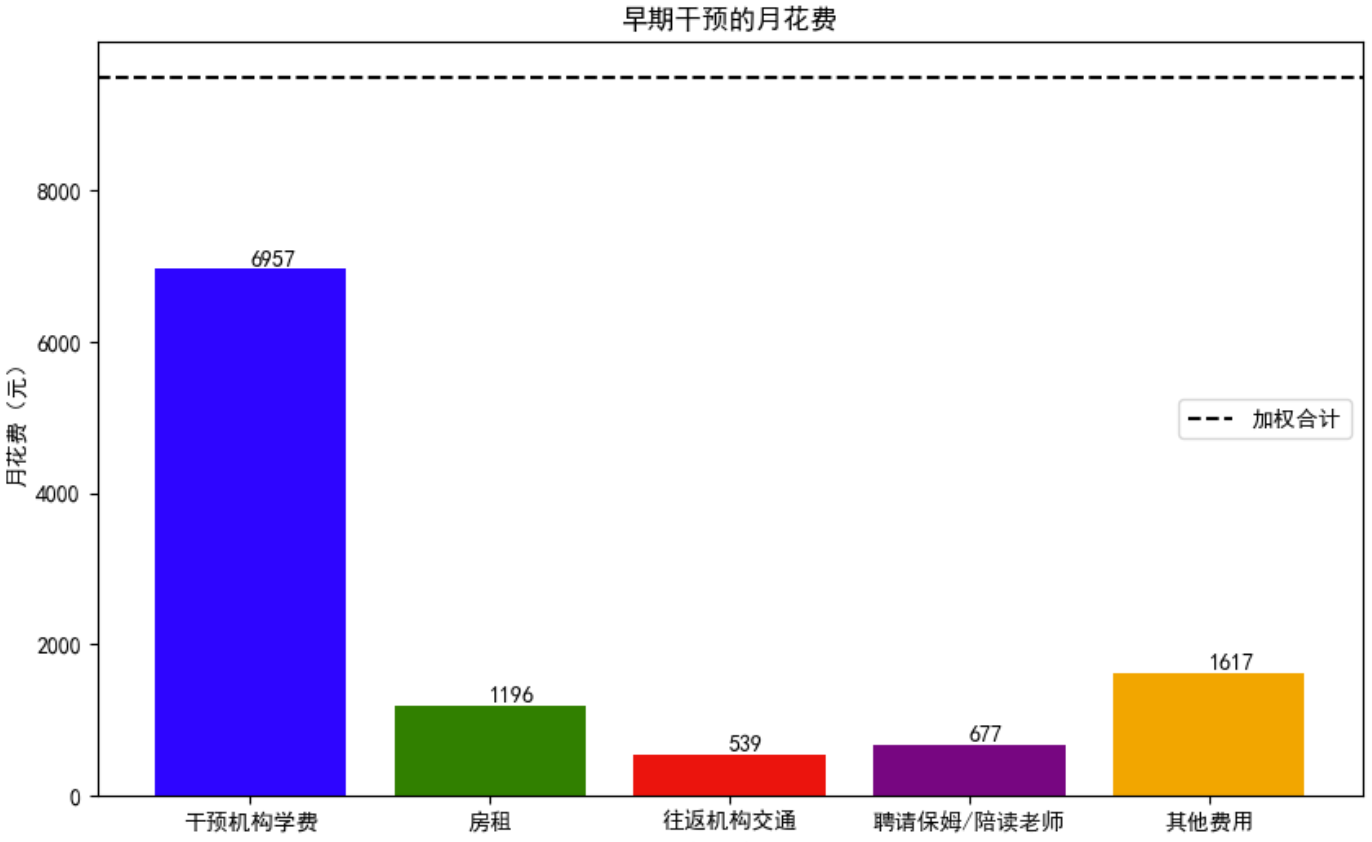
\includegraphics[width=0.85\linewidth]{include_picture/孤独症家庭每月用于干预的费用.png}
    \caption{孤独症家庭每月用于干预的费用}
    \label{fig:beichen-cost}
\end{figure}

其二，专业干预资源总量不足且地区分布不均。全国平均医患比为 1:132，省会城市每万名儿童拥有的干预师数量约为县域地区的 6.8 倍，城乡及不同地区之间的专业干预服务可及性因此存在明显差异；其三，长期照护还会影响家庭成员的就业与生活安排。相关调查显示，23.4\% 的家庭存在主要成员退出劳动力市场、承担全职照护的情况，该决策虽能提升干预持续性，却使家庭抗风险能力下降 47\%，且主要照料者出现临床抑郁症状的比例达普通人群的 3.2 倍。

\begin{figure}[H]
    \centering
    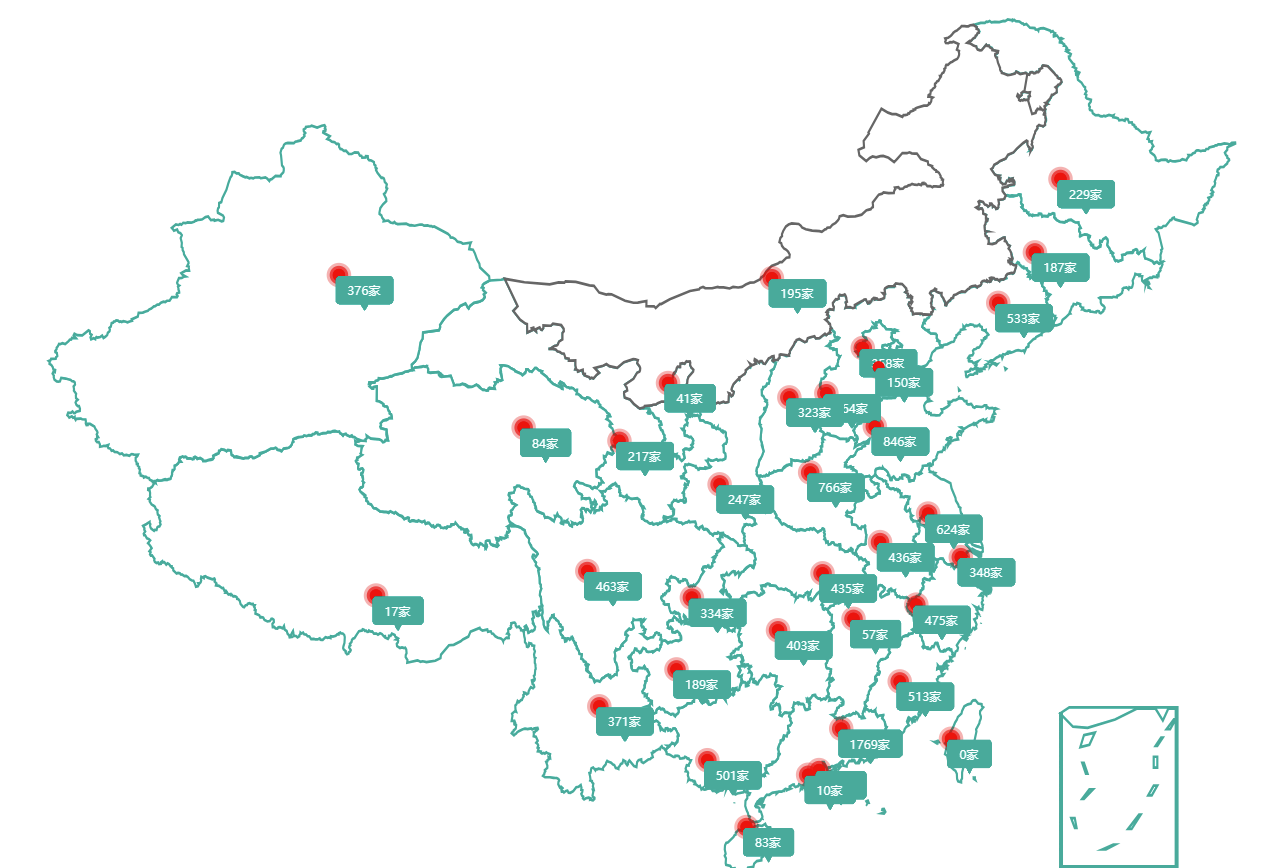
\includegraphics[width=0.72\linewidth]{include_picture/我国孤独症干预机构分布.png}
    \caption{我国孤独症干预机构分布}
    \label{fig:beichen-institutions}
\end{figure}

从现有服务实践来看，家庭经济负担与机构承载能力仍是影响长期干预的重要因素。家庭负担较重、专业机构承载能力有限等问题，会直接影响干预服务的可及性和持续性。因此，如何在专业机构干预之外拓展家庭和社区训练场景，降低持续训练的时间和资源成本，是当前孤独症儿童干预面临的重要现实问题。

\subsubsection{虚拟现实技术辅助孤独症干预}

虚拟现实技术拥有得天独厚的优势。依托多维感知重构和沉浸式场景模拟，它可将公共出行、购物、课堂互动和日常沟通等现实中组织成本较高、风险较难控制或不易反复练习的生活情境，转化为可控制、可分级、可重复的训练任务。专业人员可围绕儿童的训练目标，灵活设定场景人物、环境刺激、交互节奏与任务难度，使儿童在熟悉、可预测的环境中逐步练习社会沟通、情绪识别和日常生活技能，并将获得的经验迁移至真实生活。相较于以线下单一情境为主的训练，VR 还可在同一框架下提供多次、稳定且难度递进的练习，更好地适应儿童在参与节奏和支持方式上的个体差异。

沉浸式交互能够增强训练的参与感，并连续记录儿童在任务中的注视、反应、语言表达和完成情况，为个体化方案的制定与动态调整提供过程依据。截至 2026 年，空间计算、6DoF 追踪、眼动交互、三维语义分割、神经渲染和多模态生成式人工智能的发展，进一步丰富了个体化训练场景的构建方式。以 3D Gaussian Splatting 为代表的显式三维表示可在较短时间内实现高质量、实时的场景渲染[25]；结合语义分割，可将家庭或机构中的目标物体转化为可配置的训练元素。语音识别、语音合成与受控对话模型则可支持脚本化提示、角色扮演和训练记录，使训练内容更贴近儿童的真实生活经验。

现有研究已开始验证 VR 在孤独症儿童社交互动、情绪调节和日常技能训练中的应用效果。2026 年的系统综述汇集 22 项沉浸式或可穿戴 VR 研究，结果表明，VR 在社交互动、情绪调节和日常技能训练中展现出良好的应用前景[54]。头显眼动还可为注视目标、共同注意和任务完成过程提供量化线索，帮助专业人员更细致地观察儿童在训练中的行为变化，并据此优化训练内容与支持策略[55]。

由于训练过程涉及未成年人的人像、语音、眼动及家庭场景数据，相关应用还需同步考虑数据安全与隐私保护要求[57]。因此，VR 为训练场景的重复构建、个体化配置和过程记录提供了技术基础，并为机构训练向家庭场景延伸提供了新的实现方式。

\section{相关研究}

\subsection{虚拟现实技术在孤独症干预领域进展}

\subsubsection{社交能力训练}

孤独症的核心症状之一表现为社会交往能力的功能性损伤，其病理机制涉及多模态 神经网络的异常整合[16]。Lord et al.2020 等人的研究表明，孤独症个体在联合注意、情 绪识别及互动式对话等社交场景中普遍存在显著缺陷：约 89\%的学龄期患者无法维持 持续目光接触，72\%存在非语言交流（如手势、表情）解码障碍[17]

近年来，虚拟现实（VR）技术在自闭症谱系障碍社交能力干预领域展现出显著潜力。Ke 等针对 9--11 岁孤独症儿童开发了基于目标导向的 VR 社交训练系统[18]，其创新性体现在将任务结构划分为问题解决（如逻辑推理任务）与自主决策（如开放式社交探索）两大模块。该系统通过个性化动态算法与标准化协议的结合，重点培养儿童在人际互动中的反应启动、任务协商及自我表达等核心能力。研究者采用家长报告的标准化量表（SCQ 与 SSQ）进行前后测评估，结果显示干预后 SCQ 得分显著降低（$P=0.01$），表明社交沟通障碍得到缓解；SSQ 得分则出现统计学显著提升（$P<0.05$），证实社交技能获得系统性改善。该研究验证了结构化 VR 训练对孤独症儿童社交能力多维度的促进作用。

进一步研究表明，沉浸式 VR 环境的适应性设计可增强干预效果。Soltiyeva 等构建的“农场情境自适应 VR 系统”为 4--15 岁孤独症个体创设了动态社交互动场景[19]：受试者需在虚拟环境中完成与农夫角色及动物的渐进式交互任务，系统通过实时情绪识别算法调整虚拟角色的反馈模式。实验数据显示，80\% 的参与者在任务执行期间表现出持续互动动机，且两阶段任务平均得分从基线 2.83 分提升至 3.33 分（$\Delta=17.67\%$），证实系统能够有效促进孤独症儿童在陌生社交情境中的适应性表现。此类研究为开发具生态效度的数字干预方案提供了重要方法论参考。

\subsubsection{工具性生活能力训练}

孤独症儿童的核心社会认知缺陷导致其对环境线索的觉察与适应性响应存在显著 障碍，这种社会信息处理异常不仅造成日常功能独立性受损，更与意外伤害发生率升高 呈正相关。虚拟现实（VR）技术通过构建生态效度高的模拟环境，为解决上述问题提 供了创新性干预路径：其既可通过多模态感官输入促进技能迁移，又能确保训练过程的 风险可控性。在此领域，Tan 等设计的“交通安全VR 训练系统”具有代表性价值。该 研究采用多阶段干预框架，首先通过结构化课程教授交通规则认知基础[20]，随后在渐 进式难度设计的四个虚拟交通场景中实施情境化训练，最终通过标准化测试评估技能掌


握程度。实验数据显示，干预组中 60\%的孤独症儿童达到测试满分标准，其余参与者 正确率亦达80\%以上，证实该系统能有效提升目标人群的道路安全决策能力与标志识 别准确性。此研究结果从神经行为可塑性角度揭示了VR训练在促进孤独症儿童社会适 应能力和工具性生活能力发展中的潜在机制。

2026 年的系统综述纳入 22 项沉浸式可穿戴 VR 研究，显示此类技术可服务于孤独症人群的社交沟通、共同注意、情绪调节和日常生活技能训练；眼动等技术的结合，也使训练过程中的行为观察更为客观、细致[54]。这一研究趋势推动 VR 干预由预设的单一任务向高拟真场景、动态交互和个体化反馈发展。

\subsection{孤独症患者眼动分析}

韩俊霞等人针对孤独症患者的眼动追踪研究中发现孤独症组对共同注意在各个年 龄均低于正常组．孤独症组在注视背景和身体部分也明显高于正常组．在注视嘴部部分 正常组随年龄没有明显变化，而孤独症随着年龄增大,其对嘴部的注视显著增加[21]。

眼动特征分析中，共同注意是指通过跟随、引导后产生的关注，是两人对某一物体的注意能力。宫为大等人通过分析 106 名患者儿童的共同注意能力发现，孤独症患儿眼睛以及头部引导的共同注意能力较差，并且这些眼动特征与患儿社交障碍、孤独症症状具有显著关联[22]。

孤独症儿童的注视模式随年龄增长呈现动态变化，马伟娜等人的研究表明，孤独症 儿童在面部识别中更依赖嘴部信息，而典型发育儿童则偏好眼部区域，且这种差异随年 龄增长愈发明显[23]

\subsection{3D 高斯泼溅场景生成}

3D 高斯泼溅（3D Gaussian Splatting）是一种结合显式表示与隐式优化的三维重建技术，通过将场景表示为各向异性的 3D 高斯分布，实现高效渲染与高质量重建。其核心优势包括实时渲染（30 fps）和高保真视觉效果，突破了传统 NeRF 方法的效率瓶颈[24]。

Bernhard Kerbl 等人提出了3D 高斯泼溅的基础框架，通过优化高斯参数（位置、 协方差、透明度等）和自适应密度控制，实现了高效的场景建模与实时渲染[25]

Xue等人利用SAM和DINO等视觉模型生成语义掩码，通过几何复杂度正则化优 化高斯分布，实现了非结构化场景（如城市街道、自然景观）的精确分割与编辑，显著 提升了VR场景的交互体验[26]

鉴于生成的高斯泼溅场景均为点云，不同物体间耦合严重，JiazhongCen等人的工 作将 Segment Anything Model 的分割能力从 2D 掩码提炼到亲和特征中，以及采用软 尺度门机制，通过根据指定的3D物理尺度调整每个特征通道的大小来处理3D分割中 的多粒度模糊[27] [28]


\section{本项目成果与创新点}

针对孤独症患儿康复的核心手段——干预训练，本项目旨在构建拥有高保真的场景和人物的 3D 系统，从而可以直接用于孤独症患儿模拟社交和干预情景并通过模拟对患儿进行训练。在此期间，北辰着力攻破现有 VR 在孤独症干预领域存在的场景失真和人物缺乏表情等社交因素的问题，在只需要一段简单的输入视频的条件下，通过 3D 高斯技术构建高保真的场景和动态人物，并且运用实时人物重建技术，使得干预师可以远程参与到干预中，通过在 VR 中进行一系列引导操作，对患儿认知功能、社会交往、语言和与表达能力和工具性日常生活能力进行一体化干预训练。此外，针对孤独症儿童的眼镜回避现象，相比眼动分析仪，我们所构建的沉浸式眼动分析范式通过高生态效度的虚拟场景自然诱发儿童注视行为，该技术将复杂神经发育评估转化为可穿戴设备驱动的行为数据分析，为家庭化干预提供客观动态监测锚点。

\section{核心技术体系与系统优势}

\subsection{系统总体技术架构}



北辰围绕沉浸式社交干预中的环境构建、人物交互、智能对话与行为反馈四个关键环节，构建了由高保真可编辑三维场景构建、高保真人物动态重建、多模态 AI 智能交互以及 VR 眼动行为量化组成的核心技术体系。

\begin{figure}[H]
    \centering
    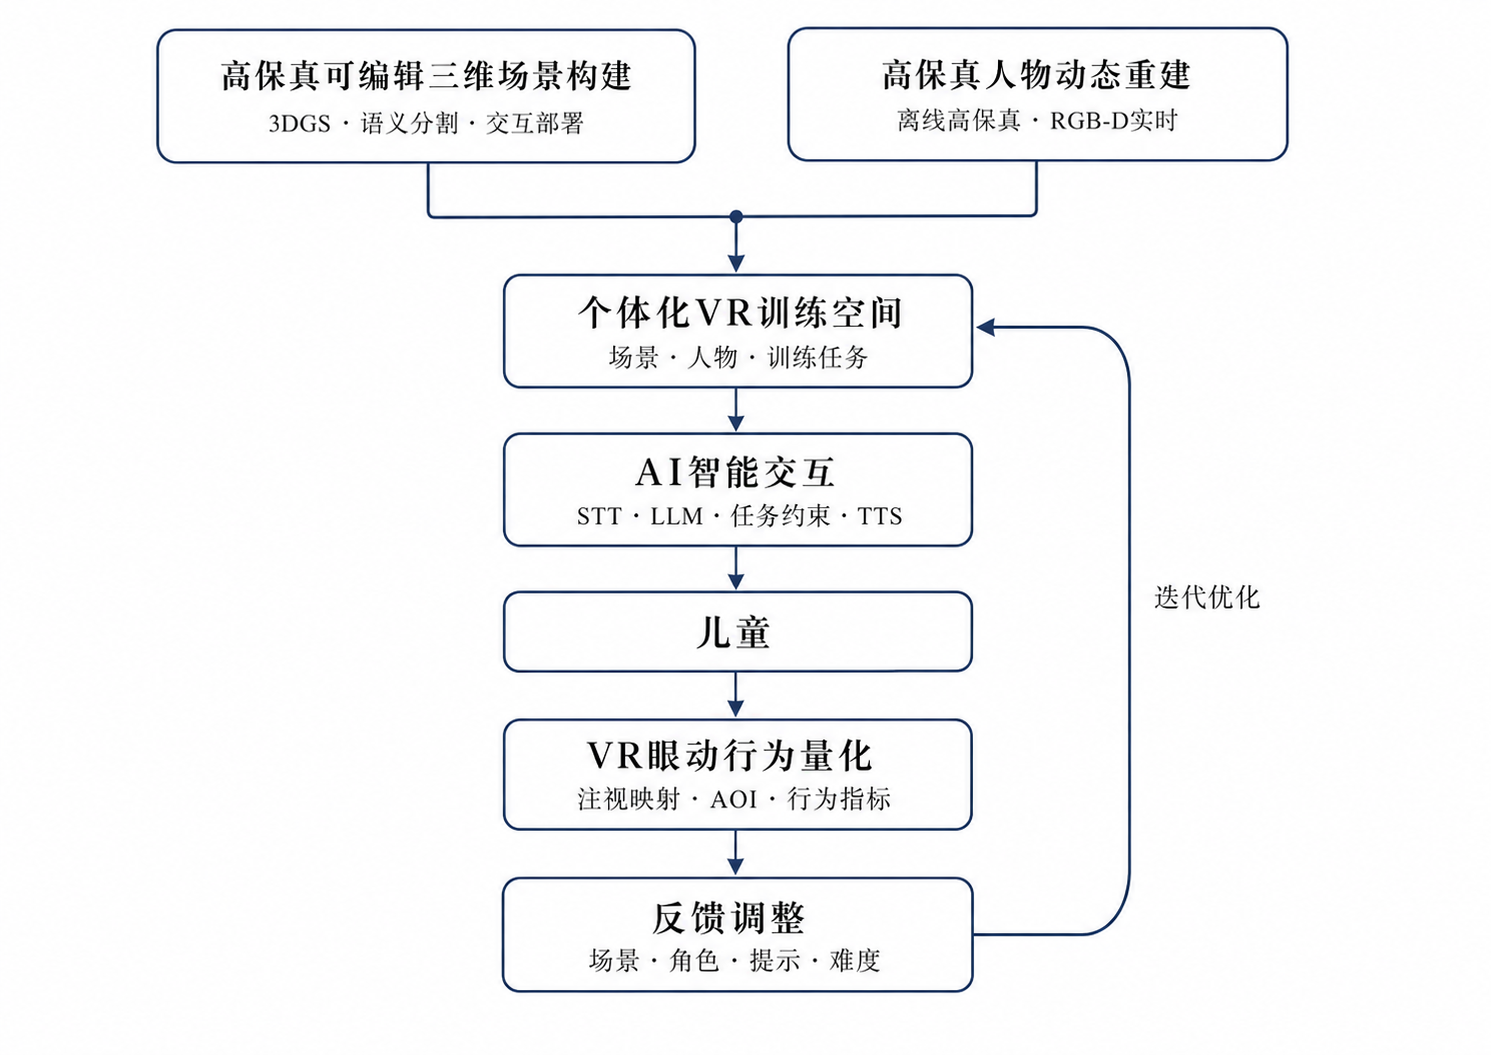
\includegraphics[width=0.88\textwidth]{technical_architecture.png}
    \caption{北辰系统总体技术架构与闭环机制}
    \label{fig:technical_architecture}
\end{figure}

如图~\ref{fig:technical_architecture} 所示，四项核心技术并非相互独立，而是围绕完整的虚拟现实社交训练过程形成协同关系。系统首先通过真实环境与人物数据构建个体化虚拟训练空间，在此基础上由 AI 驱动的虚拟角色或干预师与儿童完成既定社交任务；训练过程中，眼动模块同步记录儿童对人物、目标物体及其他关键区域的注意行为，并结合任务完成情况形成可量化的过程数据。相关结果可进一步用于调整后续训练中的场景内容、角色设置、交互提示和任务难度，从而形成“场景与人物构建—社交交互—行为采集—反馈调整”的技术闭环。


\subsection{面向交互训练的高保真可编辑三维场景构建}

虚拟现实训练首先需要解决“场景从哪里来”的问题。传统三维场景通常依赖人工建模、材质制作和场景拼装，当训练内容需要频繁更换，或希望复现儿童熟悉的家庭、学校和日常生活环境时，逐场景建模会带来较高的制作成本。因此，北辰采用视频驱动的三维场景构建路线：先利用 3D 高斯泼溅完成真实环境的高保真重建，再对场景中的目标物体进行分割和实体化处理，使原本侧重视觉呈现的重建结果进一步具备对象级编辑和交互部署能力。

\subsubsection{视频驱动的 3D 高斯场景重建}

北辰的场景构建以普通环境视频作为主要输入。相比依赖规则网格和人工材质制作的传统建模流程，3D Gaussian Splatting（3DGS）直接以大量可优化的三维高斯基元表示场景，既保留了显式表示便于快速渲染的特点，又能够通过可微优化不断逼近输入图像中的几何与外观信息[29,30]。对于需要在 VR 中反复加载和观察的真实生活场景，这种表示方式能够兼顾视觉保真度与渲染效率，因此被选作北辰场景数字化的基础表示。

每个三维高斯基元由位置、尺度、旋转、不透明度和颜色等属性共同描述。其中，位置由三维坐标 $(x,y,z)$ 确定，对应高斯分布中心 $\mu$；基元在空间中的形状和方向则由协方差矩阵 $\Sigma$ 控制。为保证矩阵在优化过程中的有效性，将其分解为旋转矩阵 $R$ 与尺度矩阵 $S$：  

\begin{equation}
\Sigma = R S S^{T} R^{T}
\end{equation}

这种分解将高斯基元的旋转与各轴尺度分别参数化，使不同高斯可以根据局部几何结构形成方向和尺度各异的椭球。对于桌面、墙面、树木以及具有复杂边缘的室内外物体，不必强行使用统一形状描述，场景细节可以由大量各向异性高斯共同逼近。其空间表示形式如图~\ref{fig:beichen-anisotropic-gaussian} 所示。

\begin{figure}[H]
    \centering
    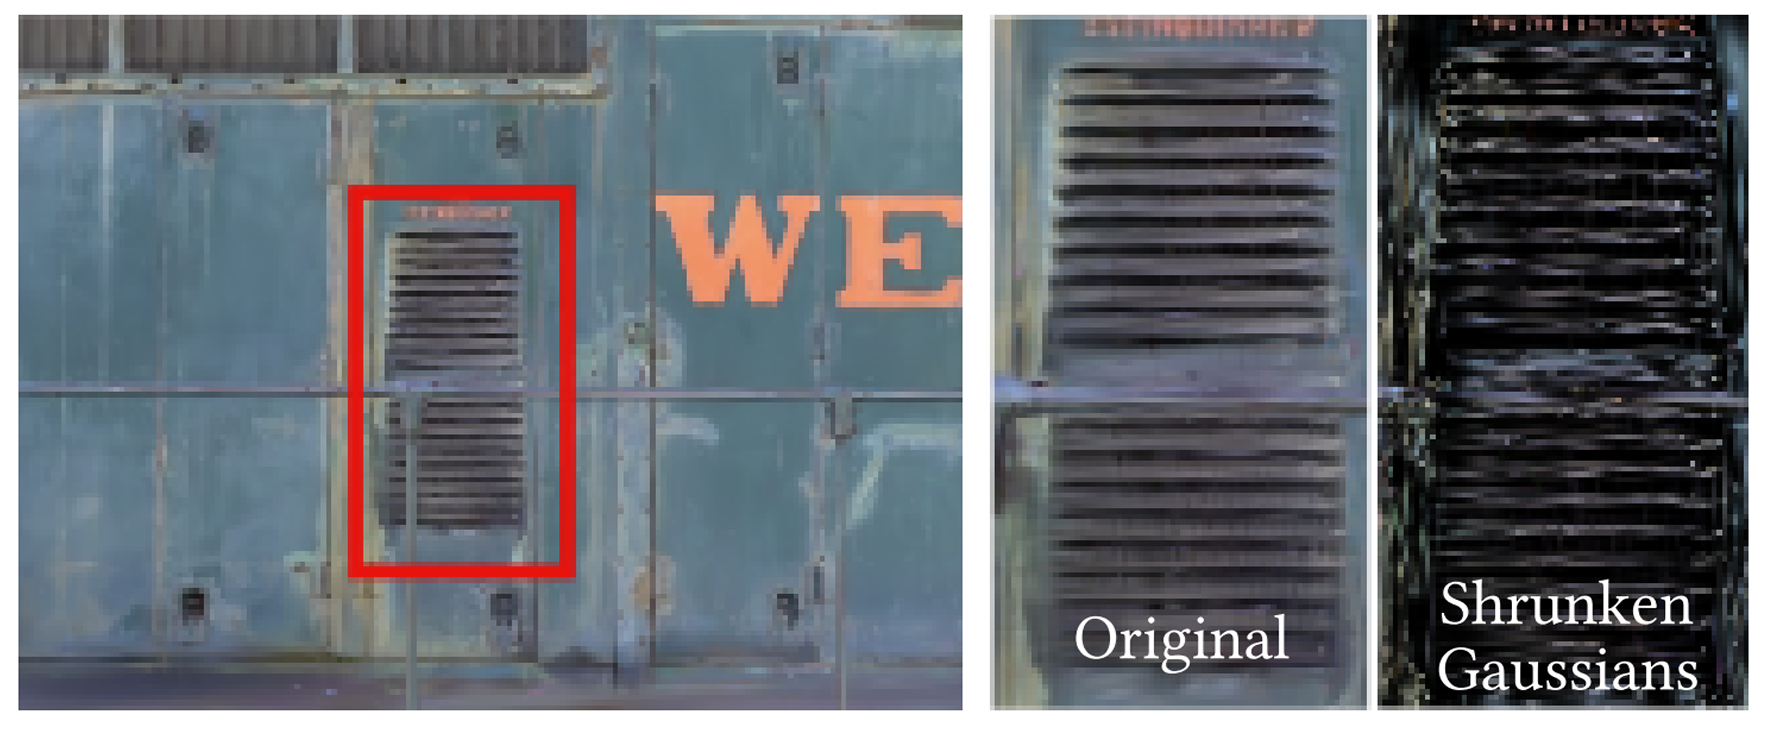
\includegraphics[width=0.78\linewidth]{include_picture/各向异性形状的高斯.png}
    \caption{各向异性形状的高斯}
    \label{fig:beichen-anisotropic-gaussian}
\end{figure}

优化过程中同时调整三维位置、不透明度 $\alpha$、各向异性协方差 $\Sigma$ 以及描述视角相关颜色的球谐（SH）系数，并结合自适应密度控制提高复杂区域的表示能力[32]。图像重建损失由像素级 $L_1$ 损失和结构相似性损失共同构成：

\begin{equation}
L=(1-\lambda)L_1+\lambda L_{D-SSIM}
\end{equation}

其中，$L_1$ 衡量渲染图像与真实图像之间的像素差异，$L_{D-SSIM}$ 则由结构相似性指标 SSIM 构造，用于约束亮度、对比度和局部结构的一致性。两类损失共同作用，使优化过程既关注局部像素误差，也兼顾整体视觉结构。

为提高训练与渲染效率，系统利用 CUDA 对高斯投影、排序和像素级 $\alpha$ 混合等计算进行并行化处理。渲染时，三维高斯根据当前相机参数投影至图像平面，并按照深度关系参与像素颜色累积。大量高斯基元的计算可在 GPU 上并行完成，从而降低复杂场景的渲染开销，为后续 VR 场景部署提供性能基础[33]。

场景重建实验在 Ubuntu 22.04 LTS 环境下完成，计算平台配备两块 NVIDIA GeForce RTX 3090 Ti GPU，并采用 CUDA 11.8 进行并行加速。该配置主要用于高斯参数优化及场景渲染测试，后续各项重建时间均基于上述实验环境记录。  

\begin{figure}[H]
    \centering
    \begin{subfigure}[b]{0.45\textwidth}
        \centering
        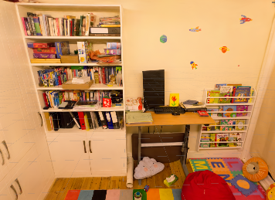
\includegraphics[width=\linewidth]{include_picture/场景 1-书房.png}
        \caption{场景1-书房}
    \end{subfigure}
    \hfill
    \begin{subfigure}[b]{0.45\textwidth}
        \centering
        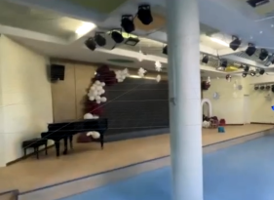
\includegraphics[width=\linewidth]{include_picture/场景 2-舞台.png}
        \caption{场景2-舞台}
    \end{subfigure}

    \vspace{0.5em}

    \begin{subfigure}[b]{0.45\textwidth}
        \centering
        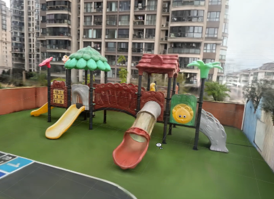
\includegraphics[width=\linewidth]{include_picture/场景 3-室外滑梯.png}
        \caption{场景3-室外滑梯}
    \end{subfigure}
    \hfill
    \begin{subfigure}[b]{0.45\textwidth}
        \centering
        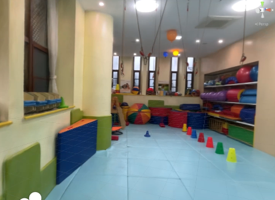
\includegraphics[width=\linewidth]{include_picture/场景 4-游戏室.png}
        \caption{场景4-游戏室}
    \end{subfigure}
    \caption{3D 高斯泼溅场景展示}
    \label{fig:beichen-scenes}
\end{figure}

从不同室内外场景的重建结果可以看出，该方法能够较完整地恢复环境中的主要空间结构、物体外观和复杂纹理，为下一步对象级分割提供统一的三维表示基础。


\subsubsection{基于亲和特征的三维物体语义分割}

完成场景重建并不意味着场景已经可以直接用于交互。原始 3DGS 中，大量高斯基元共同构成连续的视觉表面，一张桌子、一个玩具以及周围背景在数据结构上仍属于同一组场景表示。它适合“看”，却不天然知道哪些高斯属于同一个物体。对于 VR 训练而言，如果无法把目标物体从背景中独立出来，就难以继续进行对象级编辑和后续交互设置。因此，北辰在高斯场景重建基础上进一步加入三维物体分割过程。  

为获得对象级表示，我们为每个 3D 高斯附加亲和特征向量，并通过尺度门控机制控制不同特征通道在不同物理尺度下的响应[27,36,37]。对于大小差异明显的物体，固定尺度容易将局部结构过度拆分，或者把相邻对象错误合并。尺度门允许系统根据当前指定的三维尺度选择更合适的特征子空间，从而缓解多粒度场景中的分割歧义。由于同一尺度门可以作用于各高斯的亲和特征，因此特征可先随高斯一起投影至二维，再完成尺度调制：

\begin{equation}
F^s(p)=S(s)\odot F(p)
\end{equation}

\begin{equation}
F(p)=\sum_{i=1}^{|g_p|}f^g_{ip}\alpha^g_{ip}\prod_{j=1}^{i-1}\left(1-\alpha^g_{jp}\right)
\end{equation}

我们发现，单纯依赖单个高斯的特征仍可能受到离散噪声和边缘区域不稳定的影响，因此进一步利用 K 近邻关系对局部特征进行平滑，使空间位置相近且具有相似语义的高斯获得更连续的特征表示。同时加入特征范数约束，减小三维特征与二维渲染特征之间的表示偏差[38]。经过上述处理后，同一目标对应的高斯能够形成较连续的对象区域，而背景及相邻物体则被进一步区分。  

\begin{figure}[H]
    \centering
    \begin{subfigure}[b]{0.45\textwidth}
        \centering
        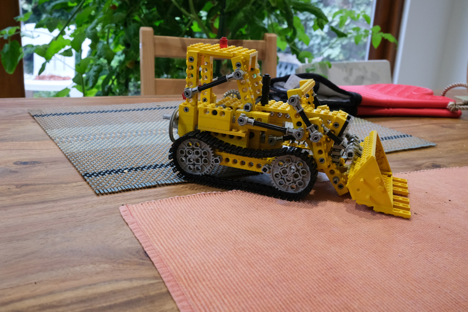
\includegraphics[width=\linewidth]{include_picture/初始未分割点云物体.png}
        \caption{初始未分割点云物体}
    \end{subfigure}
    \hfill
    \begin{subfigure}[b]{0.45\textwidth}
        \centering
        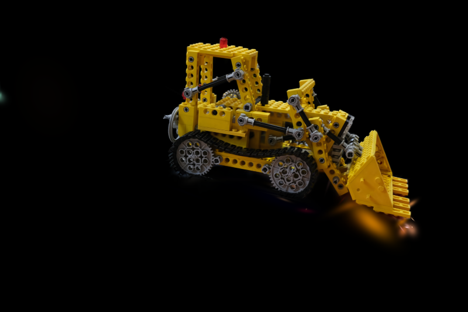
\includegraphics[width=\linewidth]{include_picture/掩码覆盖的分割物体点云.png}
        \caption{掩码覆盖的分割物体点云}
    \end{subfigure}
    \caption{物品分割前后对比}
    \label{fig:beichen-segmentation}
\end{figure}


\subsubsection{分割物体的实体化填充与交互部署}

分割得到的对象仍由高斯基元组成。它能够保持原场景的视觉外观，但本质上仍更接近由离散高斯形成的表面表示，并不等同于具有完整几何结构的实体模型。若直接将其作为 VR 交互对象，碰撞、抓取以及位置调整等操作并不方便。因此，在完成对象分割后，还需要对承担训练任务的关键物体进行实体化处理。

北辰目前采用 Unity 作为交互场景的部署平台。根据分割结果所提供的目标范围和外形，在 Unity 中选取与目标几何形态相匹配的基础模型，并通过尺度调整、组合和空间对齐对目标内部区域进行填充。这样既保留外层 3D 高斯所提供的真实纹理与视觉细节，又利用内部几何模型补足其实体结构，使场景从单纯的视觉重建结果转化为能够继续配置交互逻辑的训练资源。

实体化后的对象可以按照训练内容进一步配置。以日常生活训练为例，商品、桌椅或指定目标物体可以分别作为独立对象进行位置调整；场景中的目标区域也可以根据任务需要重新布置。相比将整个重建结果作为不可拆分的视觉背景，这种“高保真外观 + 对象级实体”的处理方式保留了真实环境的视觉特征，同时为后续交互任务设计留下了空间。

\subsubsection{场景构建性能验证与应用优势}

在现有实验配置下，对一段约 100 MB 的输入视频完成数据处理、高斯表示构建、参数优化、密度控制及可微渲染，单个场景的完整重建过程约耗时 40 min。该结果为现阶段样机测试中的实际记录，具体耗时仍会受到输入视频长度、帧数、场景复杂度及训练参数设置的影响。

从整个技术链路来看，这套方案的价值并不只是提高场景画面的真实感。更重要的是，真实环境可以由普通视频进入统一的三维重建流程，完成视觉重建后又能够继续进行对象分割和 Unity 端的实体化处理。场景因此不再是一张固定的三维背景，而可以围绕不同训练目标重新组织其中的关键对象。对于需要反复构建家庭、教室、商店等生活情境的训练任务，这种方式减少了对逐个场景从零开始人工建模的依赖，也为后续的个体化场景配置留下了更大的调整空间。


\subsection{面向社交干预的高保真人物动态重建}

社交训练中的人物既是交互对象，也是表情、姿态和动作等社会信息的重要载体。北辰没有采用单一的人物建模方式，而是根据人物角色和使用场景设置了两条重建路径：对于家长、教师等可提前采集的熟悉人物，采用离线动态人物重建方式，重点保留人物外观和动作过程；对于需要实时进入训练场景的远程干预师，则通过 RGB-D 深度相机持续获取彩色与深度信息，在 Unity 中实时生成三维点云人物。两条路线分别侧重重建质量和在线响应，服务于不同类型的社交训练需求。

\subsubsection{熟悉人物的离线高保真动态重建}

对于可以提前采集的熟悉人物，北辰采用离线重建方式生成动态人物序列。输入以多视角人物视频为主，首先按照时间顺序提取不同视角下的图像帧，再对人物在各时刻的三维外观与姿态进行重建。重建得到的连续三维帧可作为动态人物序列导入 Unity，并按照时间轴组织和播放。相比直接使用通用预制 Avatar，这种方式保留了实际采集人物的外观特征和原始动作过程，更适合用于父母、教师等熟悉人物的数字化呈现。

在具体的人物表示上，本项目参考 DualGS 的双高斯表示思路，将人物的运动结构与表面外观分开建模。其基本做法是使用数量较少的关节高斯描述人体整体姿态和骨骼层级运动，再利用更加密集的皮肤高斯恢复服装、皮肤以及人体表面的颜色和局部细节[39]。这种分层表示避免了由同一组高斯同时承担大尺度动作与细节外观的全部变化，也为后续连续帧中的人物运动更新提供了更清晰的结构基础。

\begin{figure}[H]
    \centering
    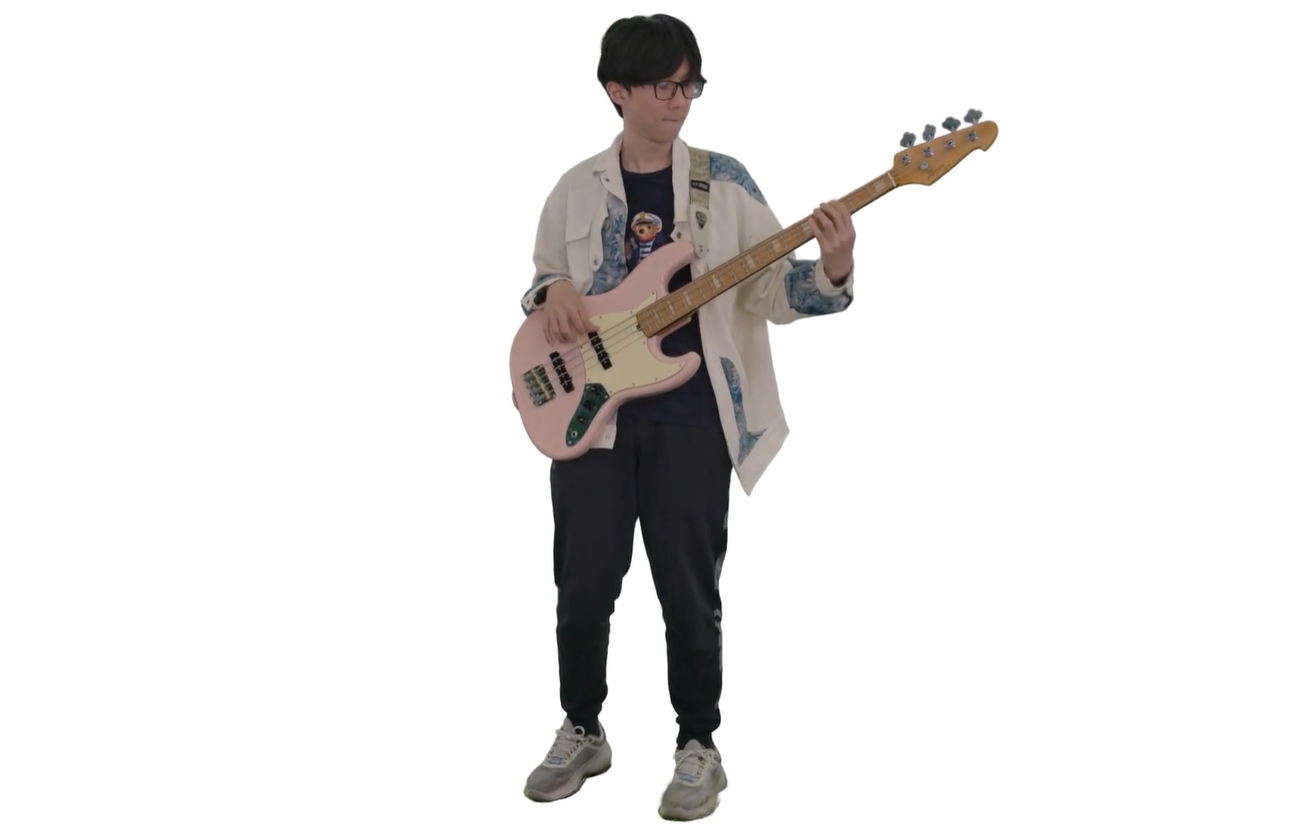
\includegraphics[width=0.42\linewidth]{include_picture/单帧 3D 动态人物重建结果.png}
    \caption{单帧 3D 动态人物重建结果}
    \label{fig:beichen-human-reconstruction}
\end{figure}

为避免人物运动与外观细节全部由同一组高斯参数承担，重建过程中采用分层的双高斯表示，将人物高斯划分为关节高斯和皮肤高斯两类。关节高斯数量较少，主要描述人物整体骨骼层级和大尺度运动，其参数重点关注关节位置 $P$ 与旋转 $Q$；皮肤高斯则更加密集，用于表达服装、皮肤及人体表面的外观细节，对应的外观属性包括球谐系数 $C$、不透明度 $\sigma$ 和尺度 $s$ 等[39--41]。

这种划分的意义在于把“人物怎么动”和“人物看起来是什么样”分开处理。动作变化首先作用于关节层级，再带动与其关联的皮肤高斯发生空间变化；皮肤高斯本身仍保留较丰富的颜色和局部外观信息。对于连续动作序列，这种层次化表示比逐帧完全独立优化更容易维持人物结构的一致性。

在现有虚拟人物的驱动中主要通过骨骼的运动来驱动虚拟人物的肢体动作，如行走、奔跑、跳跃等，使虚拟人物能够进行各种自然的动作表现[42]。点云重建中，可以借助此捕捉全局运动，如身体关节的位移和旋转使其变为一个初步的点云，骨头点云受现有虚拟人物建模中人物的驱动所启发。我们首先针对人物动作的时空特性，使用了基于物理约束的层次化运动建模方法：通过稀疏关节高斯表征骨骼层级运动，结合局部刚体变换正则化约束相邻帧间运动连续性；同时引入运动预测时序模型模块，利用历史帧速度信息预判关节位移，有效应对快速动作带来的跟踪漂移问题。这种骨骼驱动范式不仅继承了参数化模型的运动解耦优势，还通过高斯点云的显式表示突破了传统蒙皮拓扑的刚性限制。

随后我们确保了局部空间稳定性，同时通过分阶段优化策略（粗对齐与细粒度调整）实现运动与外观的显式解耦。这种分层表示提升了渲染保真度与时间一致性。

在皮肤高斯初始化阶段，引入 SMPL 参数化人体模型提供人体拓扑与姿态先验。通过人体模板与输入深度或点云信息之间的拟合，先获得较稳定的基础人体形态，再在其表面初始化并优化皮肤高斯。后续利用可微栅格化更新高斯的位置和外观参数，使其逐步逼近输入图像中的人物细节。这样做可以避免完全从无结构点云开始搜索人物形状，也便于将人物整体姿态变化与局部外观优化分开处理。最终,我们得到的是按时间组织的三维人物序列，可作为预建模角色导入后续 VR 社交场景中使用。

\subsubsection{干预师的 RGB-D 实时三维重建}

实时人物重建实验采用 Intel RealSense L515 深度相机，SDK 版本为 v2.54.2。该设备同时提供 RGB 彩色图像和深度数据，因而可以在获取人物外观纹理的同时得到对应像素的空间深度信息。

RGBD 相机能够同时获取彩色图像（RGB）和深度图像（Depth），这两种数据相互补充。彩色图像提供了丰富的纹理和外观信息，而深度图像则直接给出了场景中物体的深度信息，有助于准确地确定人物在三维空间中的位置和形状[43]。

在 Unity 端，系统首先完成深度数据与彩色图像的时间同步和坐标对齐，再依据相机内参将二维深度像素反投影至三维空间。对于深度图中的像素 $(u,v)$，其对应三维点[44]可表示为：

\begin{equation}
P(x,y,z)=K^{-1}\cdot [u,v,1]^T\cdot D(u,v)
\end{equation}

其中，$K$ 为相机内参矩阵，$D(u,v)$ 表示像素 $(u,v)$ 对应的深度值。完成反投影后，将 RGB 图像中的颜色信息映射到对应三维点，即可生成带颜色的人物点云，并在 Unity 场景中进行实时显示。

为减少背景点云进入 VR 场景，系统进一步利用深度信息进行前景范围裁剪。实际使用时，根据干预师与相机之间的工作距离设置有效深度区间，仅保留该范围内的点云数据，并过滤明显位于人物前后方的背景区域。这种方法实现简单，能够满足当前固定相机、相对受控室内环境下的人物前景提取需求。对于人物与背景距离接近或存在较大范围遮挡的情况，单纯依赖深度阈值仍可能产生误分割，后续可结合更精细的人体分割算法进一步处理。

\subsubsection{离线—在线双轨人物重建机制}

上述两类人物重建并非功能重复，而是对应不同的使用条件。家长、教师等熟悉人物通常可以提前完成影像采集，因此允许将更多计算放在训练前进行，通过离线重建获得较完整的人物外观和动作序列；远程干预师则需要在训练过程中随时进入虚拟环境，无法等待较长的离线优化，因此采用 RGB-D 相机直接生成实时点云，将重点放在动作同步和在线接入上。

基于这一差异，北辰形成了“离线预建模 + 在线实时接入”的双轨人物重建方式。前者用于构建可重复调用的熟悉人物资源，在后续训练中直接加载；后者则服务于需要干预师实时参与的训练过程。两类人物可以根据具体任务分别使用，而无需让一种重建方案同时承担高外观质量和低处理延迟两个目标。这样的划分也使人物模块与实际训练组织方式更加匹配。

\subsubsection{人物重建性能与应用优势}

当前样机已经分别完成离线人物重建结果和 RealSense L515 实时点云接入的流程验证。离线路线能够输出连续的人物高斯序列，并在 Unity 中按时间组织为动态角色；实时路线则完成了 RGB-D 数据采集、深度—颜色映射、三维点云生成以及基于深度范围的背景裁剪。两条链路均已具备进入 VR 场景的基础数据形式。

对社交训练而言，这一人物模块的价值更多体现在角色来源的扩展，而不仅是人物模型本身的视觉效果。固定虚拟角色之外，系统可以预先加入儿童熟悉的人物，也可以让远程干预师以三维形式进入训练空间，使人物配置能够随训练任务发生变化。不同角色采用不同的数字化方式，也避免了为所有使用场景重复执行同一种复杂重建流程。

\subsection{面向干预任务的多模态 AI 智能交互}

社交训练中的对话不能完全依赖固定问答脚本。儿童的表达方式、措辞和回应顺序往往并不一致，如果系统只识别少量预设句式，交互很容易中断。北辰因此在 VR 场景中接入语音识别、大语言模型和语音合成服务，将儿童的口语输入转换为文本，再结合当前训练场景与角色设定生成回复，最后重新合成为语音，由虚拟角色完成反馈。该链路的目标并不是提供开放式聊天，而是在既定训练任务内提高对话的自然度和容错空间。

项目大致流程如下：

\begin{figure}[H]
    \centering
    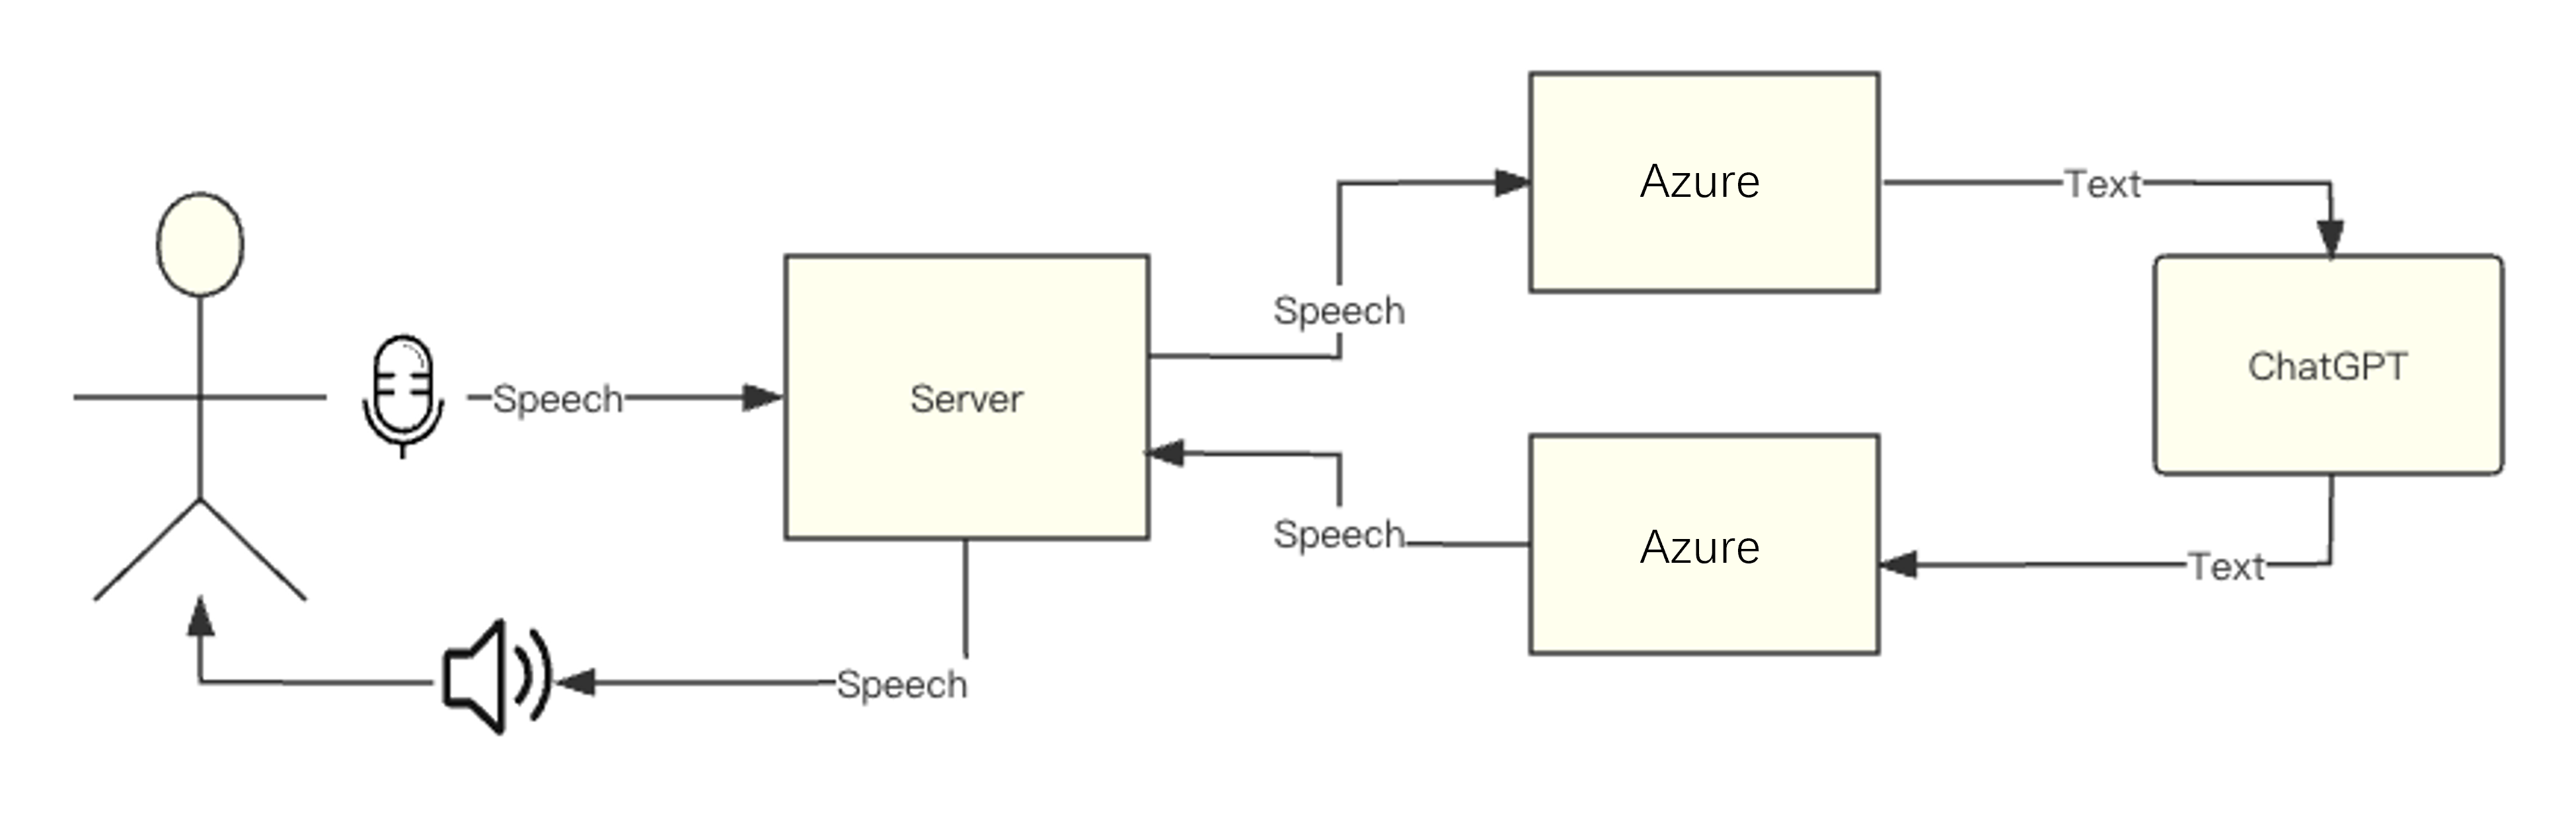
\includegraphics[width=0.82\linewidth]{include_picture/智能语音交互系统流程.png}
    \caption{智能语音交互系统流程}
    \label{fig:beichen-voice-flow}
\end{figure}

\subsubsection{语音输入输出与流式传输}

语音链路负责把儿童的口语输入送入后续对话模块，同时将模型生成的文本重新转换为可播放语音。当前系统采用 Azure Speech 提供语音转文本（Speech-to-Text，STT）和文本转语音（Text-to-Speech，TTS）能力。儿童说话后，音频首先被转换为文本并送入大语言模型；模型返回文本结果后，再由 TTS 合成为语音，在 Unity 场景中交由当前虚拟角色播放。Azure Speech 本身支持实时 STT、TTS 以及 SDK、REST API 等接入方式，能够满足这类语音应用的基本工程需求。

在 Unity 端，系统通过异步方式处理语音请求和返回结果，避免主线程因网络通信长时间阻塞。现有实现同时使用 REST API 与 WebSocket 完成不同环节的数据交互，并通过环形缓冲区管理连续音频数据，使接收和播放过程能够边到达、边处理，而不必等待整段语音全部完成后再统一播放。

\subsubsection{大模型驱动的语义理解与响应生成}

在语义响应环节，项目对 ChatGPT、ChatGLM、DeepSeek 和豆包等大语言模型进行了接入尝试。不同模型在调用成本、响应速度和语言风格上存在差异，因此系统在设计上将大模型服务与 Unity 前端解耦，前端只负责提交当前对话文本并接收返回内容，具体模型可以根据部署条件和接口可用性进行替换。对于北辰而言，大模型在该环节承担的主要任务不是医疗判断，而是理解儿童当前表达，并依据角色和训练任务生成相应的自然语言回复。

相比固定脚本，对话模型能够处理更多自然语言表达。例如儿童可能使用不同措辞表达同一意图，系统不再要求其严格匹配预设句式，而可以在语义层面对输入进行理解后给出回应。这种能力主要用于增加训练过程中的表达空间，并不替代干预师对训练目标和内容的设定。

\subsubsection{面向训练场景的任务约束型对话控制}

大语言模型可以生成较开放的内容，但开放并不等同于适合训练。北辰的对话交互仍然围绕当前 VR 场景和既定任务展开，因此需要在模型调用时加入明确的角色和话题约束，避免回复逐渐偏离训练目标。

具体而言，在发送用户输入时，系统通过 Prompt 向模型提供当前角色身份、场景背景和对话范围。例如在购物训练中，虚拟角色需要围绕商品询问、价格交流等当前任务作出回应，而不是任意切换到其他话题；在道路或课堂等场景中，则重新设置对应的角色和交流范围。这里的约束并不改变大模型本身，而是通过上下文信息限定本轮对话所处的任务边界。

\subsubsection{儿童场景下的对话安全与内容约束}

由于系统的直接使用对象包含儿童，大模型输出不能完全按照开放聊天的方式处理。当前系统在对话链路中设置了多层内容约束。首先，对进入模型的对话内容进行前置检查，减少明显偏离使用场景的请求直接进入后续生成过程；其次，通过场景焦点限制当前对话主题，使回复尽量围绕既定训练任务展开；最后，在系统 Prompt 中明确角色身份、允许讨论的内容范围和基本回复要求，从生成端进一步限制模型自由扩展话题。

这套设计的目的主要是降低回复跑题和不适宜内容进入训练过程的概率，而不是把大语言模型作为独立的安全审查或医疗决策系统。对于正式干预内容，训练任务和角色设置仍应由专业人员预先确定。

\subsubsection{低时延交互链路与系统性能}

实时语音交互的体验不仅取决于模型回复内容，也受到网络通信、语音识别、大模型推理和语音合成共同产生的等待时间影响。北辰在现有测试环境下对完整语音交互链路进行了时延测试，从语音请求发起到返回结果并进入播放流程，记录的端到端延迟控制在 730 ms 以内。该结果来自当前网络环境和服务节点下的样机测试，实际使用时仍会受到网络状况、模型接口负载以及输入语音长度等因素影响。


\subsection{基于 VR 眼动的沉浸式行为量化}

眼动追踪技术通过传感器实时监测用户的注视位置，将眼部运动转化为包含瞳距、双目注视向量和注视点的动态数据流，从而为设备提供一种新型输入方式。传统训练主要依赖干预人员现场观察，能够记录的行为细节有限。北辰因此将 VR 头显的眼动追踪能力接入训练过程，在儿童处于沉浸式场景时同步获取视线数据，并将其与当前场景中的人物和物体建立对应关系，为后续的社交注意行为分析提供数据基础。这项技术本质上依赖于传感器对眼部活动的捕捉与分析，能够将用户的视觉焦点转化为可操作的输入信号[47]。



\subsubsection{头显内嵌眼动数据采集与坐标标定}

实验中采用 PICO 4 Pro 作为 VR 显示与眼动采集设备。该头显内置双眼眼动追踪摄像头，并提供相应的 Unity 开发接口，可获得组合视线起点、视线方向及眼动数据有效状态等信息。系统在进入正式训练前完成用户眼动校准，随后在 Unity 运行过程中持续读取眼动数据，并结合头显当前姿态将视线由头显局部坐标转换到虚拟场景坐标系中，为后续注视目标判断提供统一的空间表示。  

\begin{figure}[H]
    \centering
    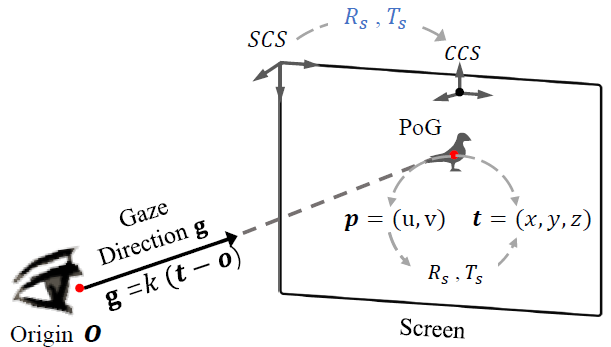
\includegraphics[width=0.72\linewidth]{include_picture/眼动分析凝视估计.png}
    \caption{眼动分析凝视估计}
    \label{fig:beichen-gaze}
\end{figure}

\subsubsection{三维注视映射与兴趣区域分析}

原始眼动数据只给出了视线在头显坐标系中的起点和方向，还不能直接回答儿童“正在看什么”。因此，系统需要将眼动数据进一步映射到当前 VR 场景。设视线起点为 $\mathbf{o}$，单位注视方向为 $\mathbf{d}$，则一条视线射线可表示为：

\begin{equation}
\mathbf{r}(t)=\mathbf{o}+t\mathbf{d}, \qquad t>0
\end{equation}

在获得头显姿态后，将视线起点与方向转换至 Unity 世界坐标系，再利用 Raycast 或相应的碰撞检测判断射线首先命中的场景对象。这样，连续的眼动向量便可以转化为“在何时注视了哪个人物或物体”的时间序列。

在得到场景对象级注视结果后，可进一步按照训练任务划分兴趣区域（Area of Interest，AOI）。例如，在人物社交任务中可以将人物面部、眼部或其他关键区域设置为 AOI；在道路和购物任务中，则可将交通信号、目标商品等任务对象设置为观察区域。AOI 并非固定不变，而是随当前训练目标进行配置。通过记录视线进入和离开这些区域的时间，可以把连续眼动轨迹整理为更容易解释的行为数据。

\subsubsection{社交注意与共同注意行为指标}

单纯保存视线坐标并不利于训练过程分析，因此需要进一步从时间序列中提取较直观的行为指标。对于指定 AOI，可以记录首次进入该区域的时间、累计注视时长、进入次数以及在总观察时间中的占比。这些指标分别反映儿童多久开始注意目标、对目标保持了多长时间，以及视线是否频繁在不同对象之间转移。

在共同注意类任务中，可将虚拟人物的视线或指向目标作为任务线索，并记录儿童是否在提示后将视线转移至对应目标区域以及完成转移所需的时间。该结果可以作为训练过程中的行为记录，用于描述儿童对共同注意线索的响应情况，而不直接作为临床诊断依据。

\subsubsection{基于行为数据的个体化反馈与训练调整}

眼动数据的价值不在于单独生成一份轨迹图，而在于帮助干预人员了解儿童在具体任务中的注意分配。例如，在人物交流任务中，如果儿童较少进入预设的人物关键区域，可以在后续训练中适当减少无关环境刺激，或调整提示对象和任务节奏；在目标搜索任务中，则可以结合目标区域的首次进入时间和停留情况，判断当前任务难度是否合适。这里的调整仍由训练人员结合任务表现进行判断，眼动数据主要提供客观的过程参考。

因此，北辰将眼动追踪定位为训练过程中的行为记录工具，而不是独立的诊断模块。它与 VR 场景最大的结合点在于，系统知道儿童当时所处的具体环境、面前有哪些人物和目标，以及任务进行到哪一步，因此同一条视线数据可以获得明确的场景语义。相比脱离任务环境单独观察眼球运动，这种同步记录方式更便于解释儿童在具体社交任务中的注意变化。北辰所强调的“沉浸式眼动”并不是更换一种眼动传感器，而是将视线记录嵌入正在进行的三维训练任务，使行为数据与场景对象、角色交互和任务阶段保持同步。


\subsection{多模态闭环干预机制与系统级技术优势}

北辰的核心技术价值并不在于单独引入某一种先进技术，而在于将三维环境重建、人物动态生成、智能语音交互以及行为数据采集连接到同一训练流程中。传统 VR 应用通常侧重视觉呈现，而固定脚本式交互又难以适应儿童在训练过程中的自然表达差异；单独的行为采集工具虽然能够记录部分指标，但缺少与具体任务场景结合的能力。北辰通过将真实环境、虚拟人物和交互数据统一到同一空间中，使训练过程中的“看到什么”“与谁交流”“如何回应”以及“产生怎样的行为变化”能够被关联记录。

在实际训练过程中，场景构建模块提供可编辑的虚拟环境基础，人物重建模块使熟悉人物或干预师能够进入训练空间，多模态交互模块负责维持自然交流过程，而眼动模块则记录儿童在任务中的注意变化。这些数据并非相互独立存在，而是围绕具体训练任务产生关联。例如，在一次人物交流任务中，系统不仅能够呈现对应场景和角色，还能够记录儿童是否关注关键人物区域、是否完成目标对象的注意转移，以及其与虚拟角色之间的交互过程。由此，训练结果不再只依赖结束时的主观评价，而能够获得更细粒度的过程数据支持。

面向孤独症儿童个体差异明显的特点，北辰所构建的技术体系提供了更灵活的训练配置方式。一方面，真实家庭、学校或公共环境可以通过三维重建转化为可调用场景，减少完全依赖人工建模的限制；另一方面，不同人物角色和交互方式可以根据训练目标进行调整。眼动行为数据则为干预人员观察儿童在具体任务中的注意表现提供客观参考。通过这些模块的结合，系统具备支持不同训练情境配置的能力，为后续开展更加针对性的社交训练提供技术基础。

从工程实现角度看，北辰当前形成了一套从环境数字化、人物生成、智能交互到行为记录的完整技术链路。相比仅提供虚拟场景体验的传统 VR 应用，该方案进一步关注训练过程中的对象交互和行为反馈；相比单纯依赖人工观察的训练方式，又增加了可重复记录的数据维度。当然，当前系统仍处于持续完善阶段，例如更大规模用户数据验证、行为指标与训练效果之间的关联分析，以及更加自动化的反馈策略仍需要进一步研究。现阶段，北辰重点实现的是一个能够支撑沉浸式社交训练和过程数据采集的技术平台。

\section{效果展示与竞品分析}

\subsection{效果展示}

\begin{figure}[H]
    \centering
    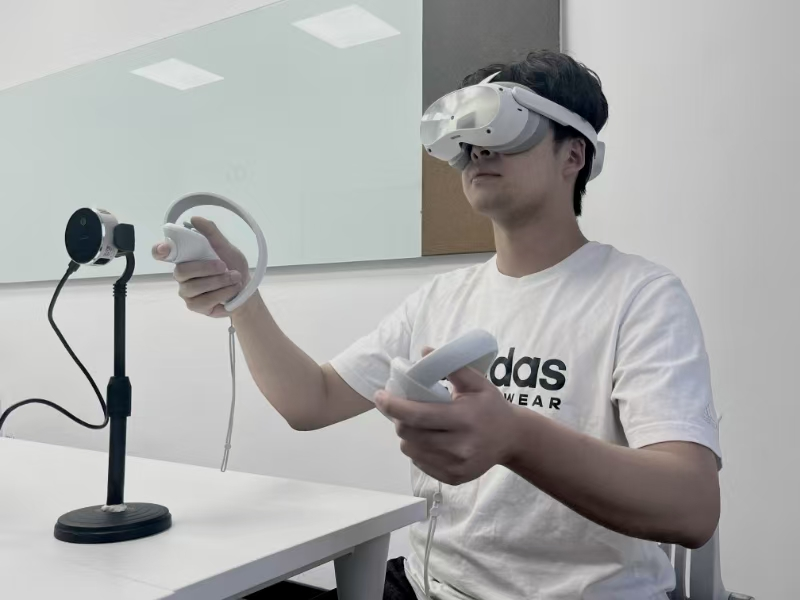
\includegraphics[width=0.58\linewidth]{include_picture/系统整体展示.png}
    \caption{系统整体展示}
    \label{fig:beichen-system}
\end{figure}

北辰充分考虑干预场景人物的真实性、社交属性、干预效果检测和个性化设置，如图 8 展示，通过在 VR 中进行一系列引导操作，对患儿认知功能、社会交往、语言和与表达能力和工具性日常生活能力进行一体化干预训练。

在认知功能方面，VR 环境提供的沉浸式体验能够有效刺激患儿的注意力和感知能力，促进其认知发展。通过高保真的 3D 高斯泼溅场景模拟真实场景和情境，患儿可以在安全的环境中进行探索和学习，从而提高其解决问题和适应新环境的能力。

\begin{figure}[H]
    \centering
    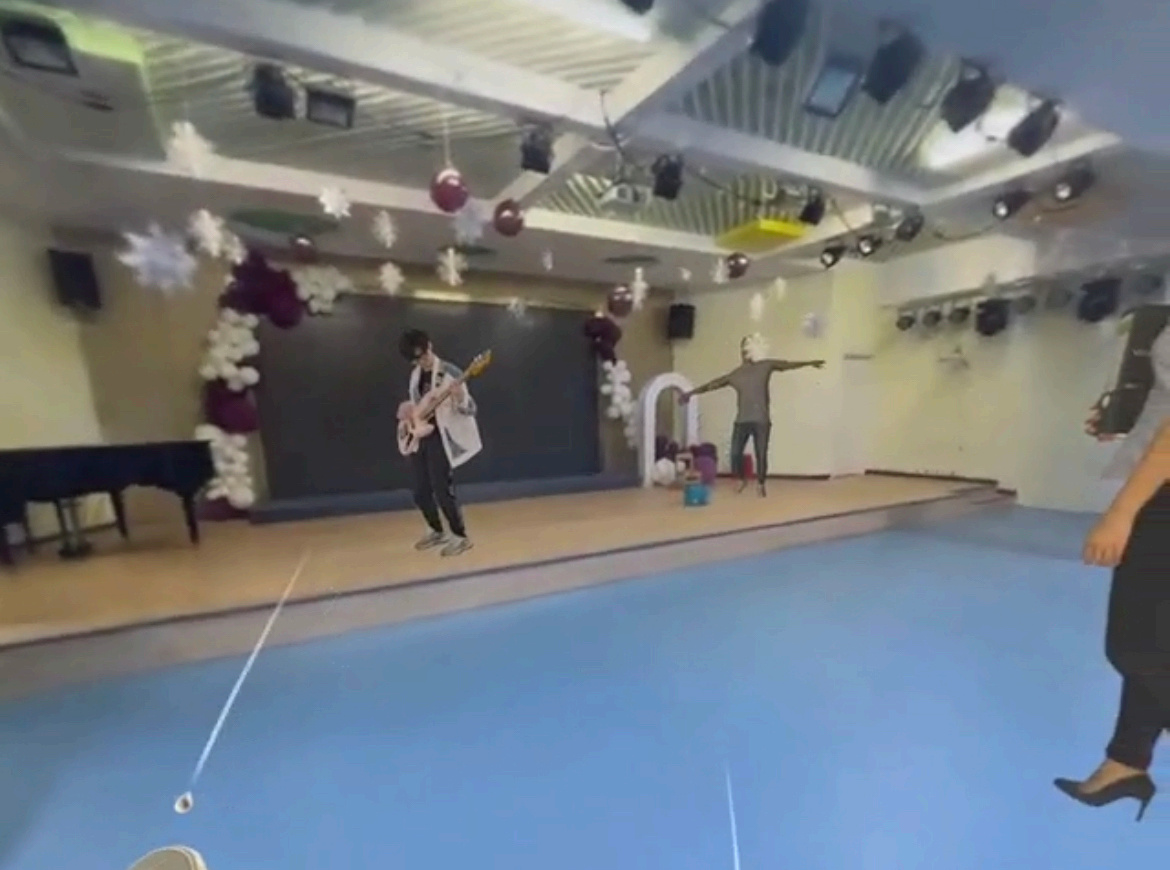
\includegraphics[width=0.72\linewidth]{include_picture/患儿视角展示.png}
    \caption{患儿视角展示}
    \label{fig:beichen-child-view}
\end{figure}

在社会交往能力的培养上，北辰利用 VR 技术创建了多样化的社交场景，如舞台、马路等，让患儿在虚拟环境中与虚拟角色进行互动。这种互动不仅能够帮助患儿理解社交规则和情感表达，还能增强其社交信心和沟通技巧，让患儿不再害怕社交，可以把学到的社交技能先在 VR 中运用上，一步步脱敏，最终可以在真实生活中去社交。

对于语言和表达能力的提升，北辰设计了特定的语言训练模块，通过多模态 AI 大模型驱动的智能语音交互系统，鼓励患儿积极表达自己的想法和感受。同时，虚拟环境中的视觉和听觉提示也为患儿提供了多感官的学习体验，有助于语言理解和表达的同步发展。

在工具性日常生活能力的训练中，北辰通过模拟日常生活中的各种情境，如购物、过马路等，让患儿在虚拟环境中练习和掌握这些技能，从而在后续生活中能够一步一步运用上这些能力。

\subsection{竞品分析}

相较于国内孤独症干预领域的先行者千丘智能与数药智能公司，以及国外的 Spirit VR 与 XR Health 公司，北辰在技术与应用方面取得了显著突破。北辰通过创新的建模技术，解决了传统建模失真的问题，同时优化了人机交互体验，为孤独症儿童提供了更加精准和高效的干预支持。此外，北辰还开发了即时构建、个性化支持和初步评估的综合解决方案，能够根据患儿的具体需求快速生成干预计划，显著提升了干预效率和效果。

与大米和小米的 AI 评估师相比，北辰还通过多模态数据的整合，进一步增强了干预方案的个性化和适应性。北辰的技术突破也为行业树立了新的标杆，推动了孤独症干预领域的技术发展，为患儿及其家庭提供了更加普惠和可持续的解决方案。

\begin{table}[H]
    \centering
    \caption{竞品分析}
    \begin{tabular}{lccc}
        \toprule
        对比维度 & 仿真评分维度 & 个性化维度 & 效果评估维度 \\
        \midrule
        千丘智能 & 40 & 不支持 & 不支持 \\
        数药智能 & 60 & 不支持 & 不支持 \\
        Spirit VR & 80 & 不支持 & 不支持 \\
        XR Health & 50 & 不支持 & 不支持 \\
        北辰 & 95 & 支持 & 支持 \\
        \bottomrule
    \end{tabular}
    \label{tab:beichen-competitors}
\end{table}

\section{商业和社会价值}

\subsection{商业价值}

\subsubsection{市场分析}

目前，孤独症干预市场前景广阔。从全球市场规模来看，如下图所示，2024 年，全球孤独症谱系障碍市场规模已达 96.18 亿美元，预计到 2031 年将增长至 120.6 亿美元，年复合增长率为 3.3\%[48]。在中国，孤独症市场规模同样呈现快速增长趋势，仅 0 到 18 岁的孤独症就已达到 96 亿元，且随着诊断水平的提高，这一规模还在快速增长。

\begin{figure}[H]
    \centering
    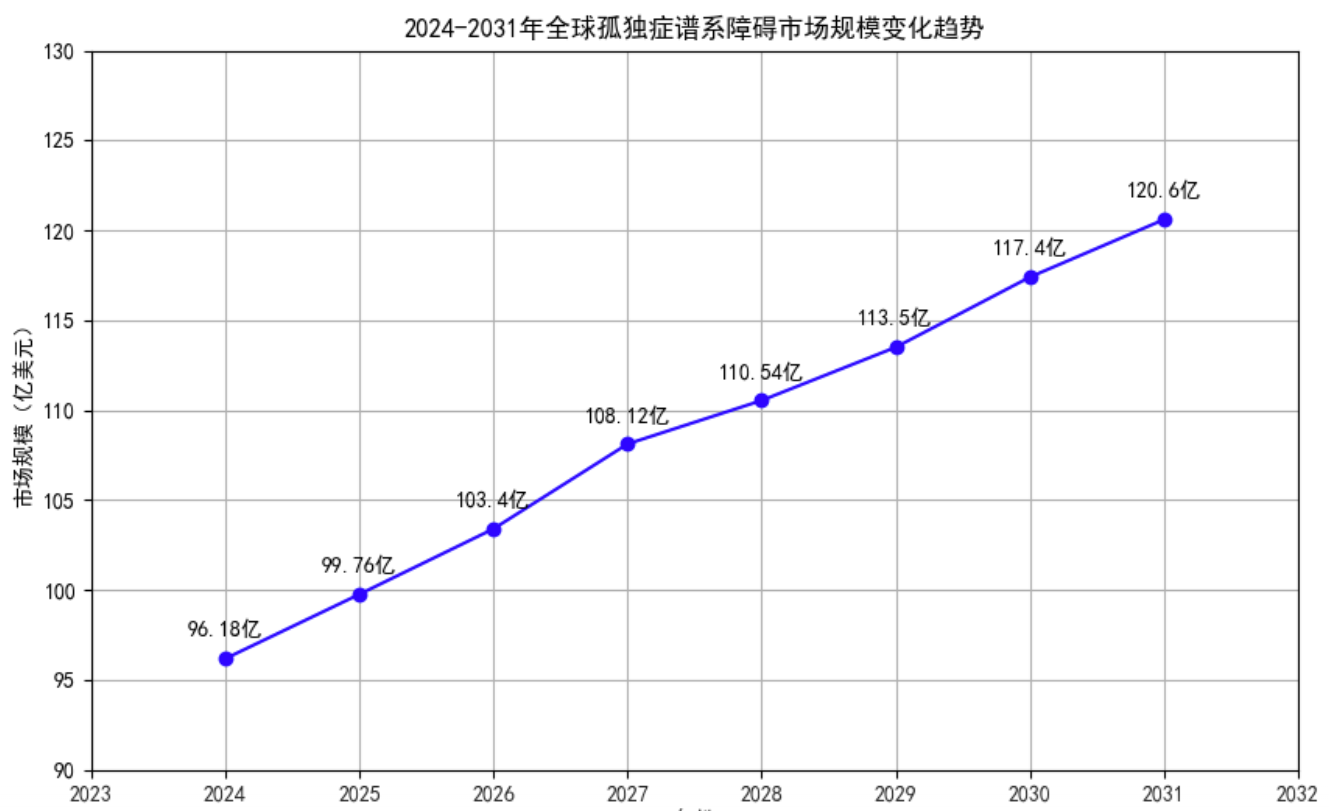
\includegraphics[width=0.80\linewidth]{include_picture/2024-2031 年全球孤独症谱系障碍市场规模.png}
    \caption{2024--2031 年全球孤独症谱系障碍市场规模}
    \label{fig:beichen-market}
\end{figure}

然而，尽管市场规模庞大，VR 技术在孤独症干预领域的渗透率仍不足 5\%，表明该技术在这一领域的应用尚处于起步阶段，具有巨大的发展潜力。北辰公司通过创新的软硬件一体式售卖模式，为患者家庭提供了更加经济实惠的干预方案，显著降低了长期干预的成本[49]。这一模式不仅使城市地区的患者家庭受益，也为偏远地区的孤独症儿童提供了接触先进康复干预的机会，进一步扩大了潜在市场规模。

北辰的技术突破和商业模式创新，有望在满足市场需求的同时，推动孤独症干预技术的普及和应用，为行业的发展注入新的活力。

\subsubsection{商业发展}

本产品定位“全球首款 AI+VR 多模态孤独症干预系统”，聚焦 3--12 岁孤独症谱系障碍儿童群体，打造“远程医疗 + 智能训练 + 精准评估”三位一体的闭环干预体系，填补现有市场在场景真实性、数据量化性和服务连续性三方面的空白。本产品具有智能性强、交互性好、高度沉浸式、成本效益佳、操作便捷的特点。在医疗服务方面，主要面向孤独症儿童及其家庭，为处于不同干预阶段的患儿提供个性化、智能化的康复训练。同时，本产品也可作为孤独症相关研究的重要工具，为科研机构提供数据支持和技术保障。本团队将以科技为核心竞争力，以满足客户需求为最终目标，通过直接面向消费者销售、与医院和康复机构合作批量销售以及向研究机构供应等多元化渠道进入市场。

作为商业产品，北辰利用上游供货商提供零件，包括但不限于 VR 眼镜、大模型服务和语音服务等，多个科研机构提供理论顾问，同时为科研机构数据支持，并面向医院、患者家庭、特殊学校进行售卖，一举实现多产业线协同发展。

商业规划方面，我们进行了长期规划，久久为功，实现商业发展“四步走”。

2025 年，北辰将完成产品研发，成立公司并通过天使轮融资为后续发展提供资金支持。同时，公司将完成产品分类界定和型式检验，确保产品符合相关行业标准，为后续市场推广奠定基础。到 2027 年，北辰计划完成 A 轮融资，进一步扩大资金储备，支持产品的规模化生产和市场推广。同时，公司将完成产品分类界定和型式检验，确保产品在市场中的合规性和竞争力。在 2029 年，北辰将推进临床评价工作，验证产品的有效性和安全性。此外，公司将深化与医院的合作，推动产品在医疗领域的应用和推广，进一步提升市场占有率。到 2032 年，北辰计划完成创新医疗器械特别审查申报，确保产品获得行业认可和市场准入资格。同时，公司将通过 B 轮融资进一步扩大资金储备，支持产品的持续研发和市场拓展。

\subsection{社会价值}

孤独症干预具有深远的社会意义，它不仅关乎个体的生活质量，更影响着家庭的幸福与社会的和谐发展。作为医疗项目，北辰一直致力于提升孤独症群体的生活质量，减轻家庭和社会的经济负担，促进社会包容和多元化发展、助力孤独症产业升级，构建孤独症产业联盟。

科技在孤独症干预中发挥着越来越重要的作用。基于“自然发展行为干预”的主流方法成为推进治疗的核心，该干预方法涉及三个关键词：自然、发展和行为[50]。即在孩子的日常生活中进行干预，针对不同年龄阶段作出个性化的支持，致力于培养健康的行为习惯，专家建议，孤独症儿童每周的干预时长应达到 25 个小时。北辰的应用使得干预更加精准、高效，也更能满足患儿的干预时间需求，为孤独症康复行业带来了新的发展机遇。

\section*{结论}
\addcontentsline{toc}{section}{结论}

在孤独症群体日益增长的背景下，本文提出优化基于虚拟现实（VR）技术辅助孤独症干预的创新路径。通过结合高保真的虚拟场景和人物，北辰能够为孤独症儿童提供沉浸式的训练体验，帮助他们在模拟的现实环境中学习社交技能、情绪管理、生活技能等多维度能力。此外，北辰允许用户自由配置训练场景和难度，支持干预效果的实时评估，从而实现个性化、精准化的干预。

与传统人为干预相比，北辰突破了地域、时间和费用的限制，为孤独症干预提供了更加高效、灵活的解决方案。例如，北辰可以模拟超市购物、公共交通出行等真实场景，为儿童提供安全可控的训练环境，同时避免现实中的不确定因素。此外，北辰的沉浸性和互动性能够显著提高儿童的学习动机和兴趣，从而提升干预效果。相比其他用于孤独症干预的 VR 产品，北辰具有明显优势。例如，通过眼动追踪、表情反馈等技术，北辰系统能够实时捕捉儿童的行为数据，为干预效果提供科学依据。同时，VR 技术的可重用性和压力调节功能使得训练更加灵活，能够逐步提升儿童的适应能力。

通过 VR 技术的赋能，我们期待为孤独症群体创造一个更加包容、多元的未来，让他们在科技的光辉中绽放光彩。万物皆有缝隙，那是光照进来的地方，北辰希望每个星星的孩子，都能成为最耀眼的那颗北辰星。

\newpage
\section*{参考文献}
\addcontentsline{toc}{section}{参考文献}

[1] 中共中央国务院. 中共中央国务院印发《“健康中国 2030”规划纲要》[A/OL]. 中国政府网, 2016. https://www.gov.cn/zhengce/2016-10/25/content\_5124174.htm.

[2] 中国政府网. 中华人民共和国国民经济和社会发展第十四个五年规划和 2035 年远景目标纲要[A/OL]. 中国政府网, 2021. \url{https://www.gov.cn/xinwen/2021-03/13/content_5592681.htm}.

[3] 新华社. 习近平：高举中国特色社会主义伟大旗帜为全面建设社会主义现代化国家而团结奋斗——在中国共产党第二十次全国代表大会上的报告[A/OL]. 中华人民共和国商务部, 2022. \url{https://m.mofcom.gov.cn/article/zt_20thCPC/toutiao/202211/20221103366898.shtml}.

[4] World Health Organization. Autism spectrum disorders[EB/OL]. World Health Organization, 2023. https://www.who.int/news-room/fact-sheets/detail/autism-spectrum-disorders.

[5] JIN L, YUEQIN H, HONG W, 等. 中国精神卫生调查报告（2019）[M]. 北京: 科学出版社, 2020.

[6] World Health Organization. 世卫组织启动委员会以促进社会联系[EB/OL]. World Health Organization, 2023. https://www.who.int/zh/news/item/15-11-2023-who-launches-commission-to-foster-social-connection.

[7] MY P. 走出孤独: 自闭症儿童的语言障碍特征分类, 评估及康复研究[D]. 吉林大学, 2016.

[8] 樊越波. 孤独症干预方法有效性循证研究述评——基于《孤独症谱系障碍循证干预指南》[J]. 残疾人研究, 2014(2): 49-53.

[9] MCNEIL C B, HEMBREE-KIGIN T L, ANHALT K. Parent-child interaction therapy[M]. Springer, 2010.

[10] WADDINGTON H, REYNOLDS J E, MACASKILL E, et al. The effects of JASPER intervention for children with autism spectrum disorder: A systematic review[J]. Autism, 2021, 25(8): 2370-2385.

[11] ROGERS S J, ESTES A, LORD C, et al. Effects of a brief Early Start Denver Model (ESDM)--based parent intervention on toddlers at risk for autism spectrum disorders: A randomized controlled trial[J]. Journal of the American Academy of Child \& Adolescent Psychiatry, 2012, 51(10): 1052-1065.

[12] GREENSPAN S, WIEDER S. DIR®/Floortime™ model[J]. The International Council on Developmental and Learning Disorders, 2008.

[13] 牛春艳. 某康复机构孤独症儿童康复效果影响因素分析[D]. 吉林大学, 2016.

[14] SHUHAIBER J H. Augmented reality in surgery[J]. Archives of surgery, 2004, 139(2): 170-174.

[15] 张思妍, 刘乐元, 陈靓影. 元宇宙赋能孤独症儿童教育干预研究初探[J]. 现代教育技术, 2025, 35(01): 128-136.

[16] 郭乃绮, 王瑜. 虚拟现实技术在孤独症谱系障碍儿童干预中的研究进展[J]. Chinese Journal of Contemporary Pediatrics, 2024, 26(4): 414.

[17] LORD C, BRUGHA T S, CHARMAN T, et al. Autism spectrum disorder[J]. Nature reviews Disease primers, 2020, 6(1): 5.

[18] KE F, MOON J, SOKOLIKJ Z. Designing and deploying a virtual social sandbox for autistic children[J]. Disability and Rehabilitation: Assistive Technology, 2024, 19(4): 1178-1209.

[19] SOLTIYEVA A, OLIVEIRA W, MADINA A, et al. My Lovely Granny’s Farm: An immersive virtual reality training system for children with autism spectrum disorder[J]. Education and Information Technologies, 2023, 28(12): 16887-16907.

[20] TAN Q P, HUANG L, XU D, et al. Serious game for VR road crossing in special needs education[J]. Electronics, 2022, 11(16): 2568.

[21] 韩俊霞, 康健楠, 欧阳高翔, 等. 孤独症儿童脑电与眼动追踪研究[J]. 科学通报, 2018, 63(15): 52-61.

[22] 宫为大, 纪红, 赵甜甜, 等. 孤独症谱系障碍患儿的眼动特征[J/OL]. 国际精神病学杂志, 2024, 51(05): 1471-1473. DOI: 10.13479/j.cnki.jip.2024.05.009.

[23] 马伟娜; 朱蓓蓓; 谢宇;. 孤独症儿童面部表情识别能力的眼动研究[J/OL]. 应用心理学, 2015, 21(1): 76. http://www.appliedpsy.cn/CN/abstract/article\_97.shtml.

[24] CHEN G, WANG W. A survey on 3d gaussian splatting[A]. 2024.

[25] KERBL B, KOPANAS G, LEIMKUHLER T, et al. 3d gaussian splatting for real-time radiance field rendering.[J]. ACM Trans. Graph., 2023, 42(4): 139-1.

[26] XUE H, JIN M, ZHANG C, et al. Image blending algorithm with automatic mask generation[C]//International Conference on Neural Information Processing. Springer, 2023: 234-248.

[27] CEN J, FANG J, YANG C, et al. Segment any 3d gaussians[A]. 2023.

[28] BARRON J T, MILDENHALL B, VERBIN D, et al. Mip-nerf 360: Unbounded anti-aliased neural radiance fields[C]//Proceedings of the IEEE/CVF conference on computer vision and pattern recognition. 2022: 5470-5479.

[29] ALIEV K A, SEVASTOPOLSKY A, KOLOS M, et al. Neural point-based graphics[C]//Computer Vision--ECCV 2020: 16th European Conference, Glasgow, UK, August 23--28, 2020, Proceedings, Part XXII 16. Springer, 2020: 696-712.

[30] BARRON J T, MILDENHALL B, TANCIK M, et al. Mip-nerf: A multiscale representation for anti-aliasing neural radiance fields[C]//Proceedings of the IEEE/CVF international conference on computer vision. 2021: 5855-5864.

[31] CHEN A, XU Z, GEIGER A, et al. Tensorf: Tensorial radiance fields[C]//European conference on computer vision. Springer, 2022: 333-350.

[32] REISER C, PENG S, LIAO Y, et al. Kilonerf: Speeding up neural radiance fields with thousands of tiny mlps[C]//Proceedings of the IEEE/CVF international conference on computer vision. 2021: 14335-14345.

[33] TAKIKAWA T, EVANS A, TREMBLAY J, et al. Variable bitrate neural fields[C]//ACM SIGGRAPH 2022 Conference Proceedings. 2022: 1-9.

[34] BOTSCH M, HORNUNG A, ZWICKER M, et al. High-quality surface splatting on today’s GPUs[C]//Proceedings Eurographics/IEEE VGTC Symposium Point-Based Graphics, 2005. IEEE, 2005: 17-141.

[35] BHALGAT Y, LAINA I, HENRIQUES J F, et al. Contrastive lift: 3d object instance segmentation by slow-fast contrastive fusion[A]. 2023.

[36] YIN X, GOUDRIAAN J, LANTINGA E A, et al. A flexible sigmoid function of determinate growth[J]. Annals of botany, 2003, 91(3): 361-371.

[37] HAN J, MORAGA C. The influence of the sigmoid function parameters on the speed of backpropagation learning[C]//International workshop on artificial neural networks. Springer, 1995: 195-201.

[38] KERR J, KIM C M, GOLDBERG K, et al. Lerf: Language embedded radiance fields[C]//Proceedings of the IEEE/CVF International Conference on Computer Vision. 2023: 19729-19739.

[39] JIANG Y, SHEN Z, HONG Y, et al. Robust dual gaussian splatting for immersive human-centric volumetric videos[J]. ACM Transactions on Graphics (TOG), 2024, 43(6): 1-15.

[40] HU S, HU T, LIU Z. Gauhuman: Articulated gaussian splatting from monocular human videos[C]//Proceedings of the IEEE/CVF conference on computer vision and pattern recognition. 2024: 20418-20431.

[41] JIANG Y, SHEN Z, WANG P, et al. Hifi4g: High-fidelity human performance rendering via compact gaussian splatting[C]//Proceedings of the IEEE/CVF conference on computer vision and pattern recognition. 2024: 19734-19745.

[42] KWON Y, LIU L, FUCHS H, et al. Deliffas: Deformable light fields for fast avatar synthesis[J]. Advances in neural information processing systems, 2023, 36: 40944-40962.

[43] KESELMAN L, ISELIN WOODFILL J, GRUNNET-JEPSEN A, et al. Intel realsense stereoscopic depth cameras[C]//Proceedings of the IEEE conference on computer vision and pattern recognition workshops. 2017: 1-10.

[44] ARKO S S H, HOSSAIN M T, DIPTO S M, et al. Real world objects augmentation in virtual 3D environment RealSense SDK, Deep Learning and Game Engine[C]//2021 IEEE Asia-Pacific Conference on Computer Science and Data Engineering (CSDE). IEEE, 2021: 1-6.

[45] GOVINDARAJU V. Locating human faces in photographs[J]. International Journal of Computer Vision, 1996, 19(2): 129-146.

[46] LIUSIE A, MANAKUL P, GALES M J. Llm comparative assessment: Zero-shot nlg evaluation through pairwise comparisons using large language models[A]. 2023.

[47] WANG Z, LU F. Tasks Reflected in the Eyes: Egocentric Gaze-Aware Visual Task Type Recognition in Virtual Reality[J]. IEEE Transactions on Visualization and Computer Graphics, 2024.

[48] BRODERICK A A. The autism industrial complex: How branding, marketing, and capital investment turned autism into big business[M]. Myers Education Press, 2022.

[49] 汤兆云, 刘科成. 我国孤独症儿童群体的社会现状、现实困境与优化治理[J]. 深圳大学学报 (人文社会科学版), 2023, 40(06): 90-99.

[50] SCHREIBMAN L, DAWSON G, STAHMER A C, et al. Naturalistic developmental behavioral interventions: Empirically validated treatments for autism spectrum disorder[J]. Journal of autism and developmental disorders, 2015, 45: 2411-2428.

\end{spacing}
\end{document}
